\section{Recognizing observed actions}
\label{sec:recognition}

The recognition of actions in videos is a fundamental computer vision research theme. Recognition tasks focus on different aspects of the actions observed in full. We start by discussing approaches for optimizing model inputs in \Cref{sec:recognition::inputs}. We then overview popular temporal-based recognition tasks in \Cref{sec:recognition::temporal}. Tasks based on the semantic relationships between language and video are discussed in \Cref{sec:recognition::language}, whereas audio-visual and other multi-modal approaches appear in \Cref{sec:recognition::audio}. %Finally, we discuss objectives and methods of recognition of approaches focusing on human-human and human-object interactions in \Cref{sec:recognition::interaction}.


\subsection{Video reduction methods}
\label{sec:recognition::inputs}

% Why sample/reduce compute?
%Based on a 2024 study \citep{sandvine2024global}, video accounts for over 5 exabytes of the world's daily internet traffic.
Video inputs typically consist of tens to hundreds of frames, with highly correlated visual characteristics. The uniform use of all frames can lead to an unsustainable computational burden. However, humans process stimuli selectively \citep{eagleman2010does}. %A class of psychophysical studies in human cognition \citep{morrone2005saccadic,wang2012life} has shown that the perception of time can be distorted; e.g. events may feel like occurring slower in brief dangerous events.
Several recognition approaches in computer vision aim at reducing compute costs to improve memory utilization by considering inputs selectively.


% Main challenges in input reduction
\subsubsection{Challenges}
 

%Frames in videos introduce redundancies. 
Reducing frame-level redundancies in videos requires a high-level understanding of temporal segments' relevance. The distinction of relevant segments and, subsequently, the selection or compression of frames, directly impacts information loss. Long and complex scenes present significant challenges to video reduction methods. This \textit{uneven context inclusion} requires more efficient utilization of the model's capacity.

\begin{figure}[t]
     \centering
     \begin{subfigure}[b]{0.49\linewidth}
         \centering
         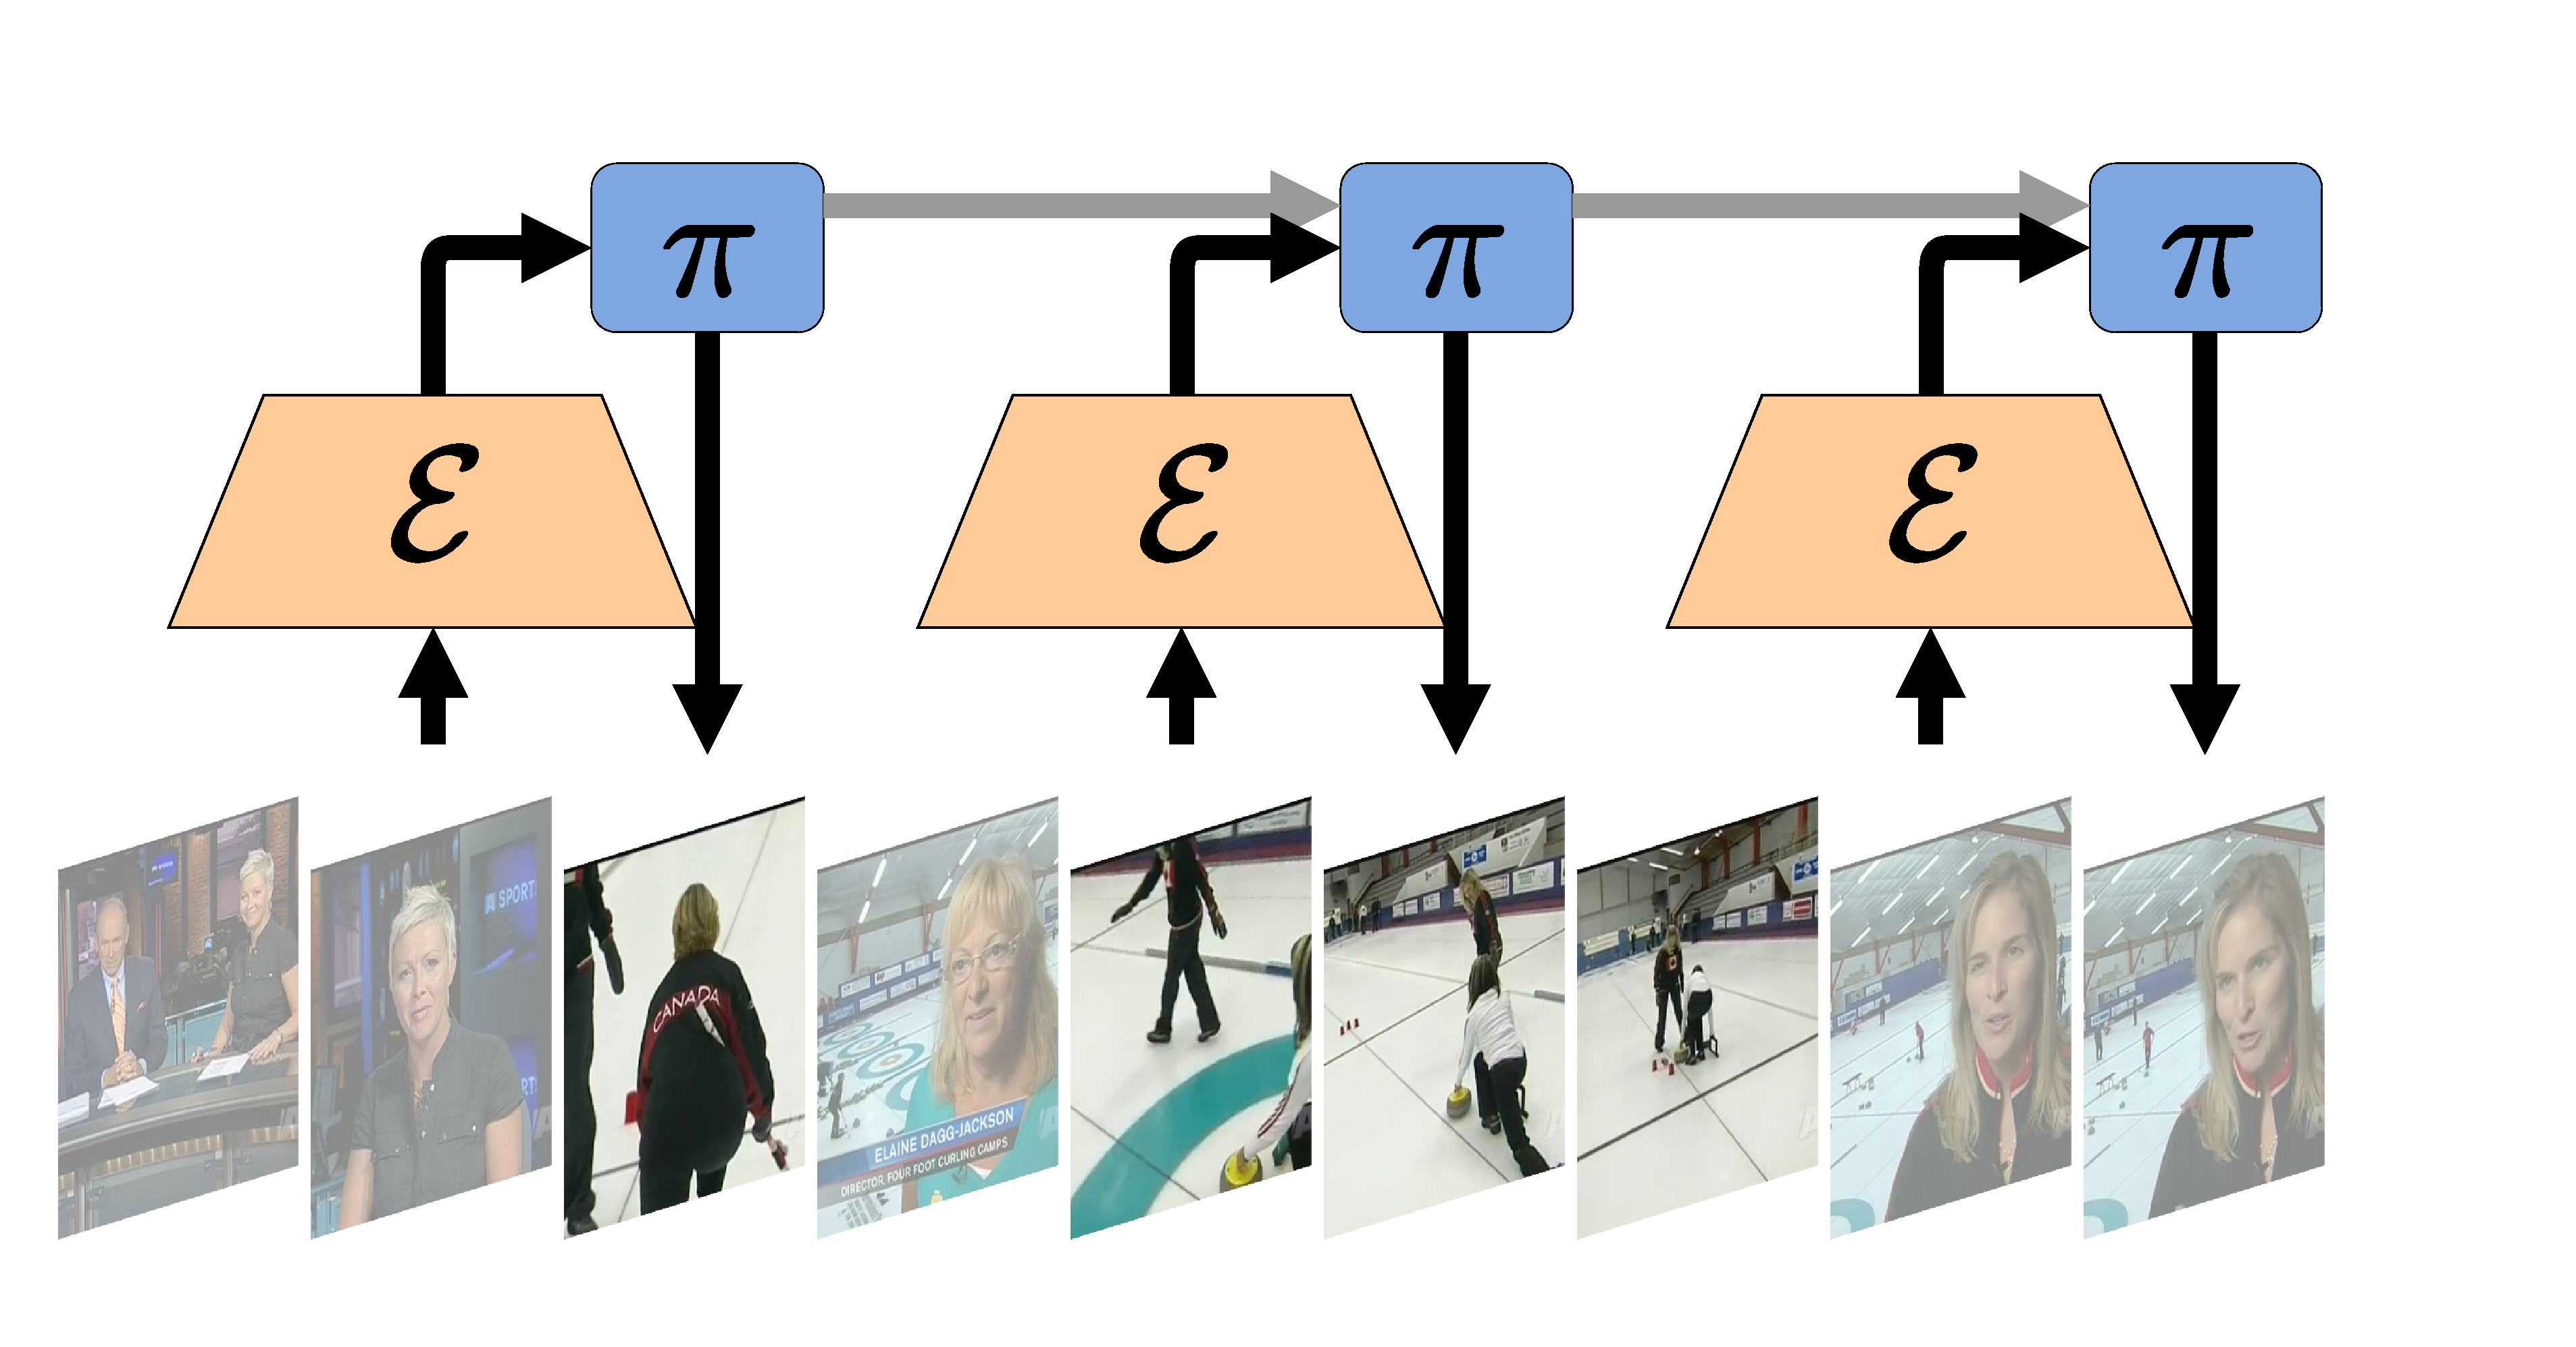
\includegraphics[width=\linewidth]{figs/redundancies_reduction/redudancies_sample.pdf}
         \caption{\textbf{Frame Sampling}}
         \label{fig:redundancies_reduction::sampling}
     \end{subfigure}
     \hfill
     \begin{subfigure}[b]{0.49\linewidth}
         \centering
         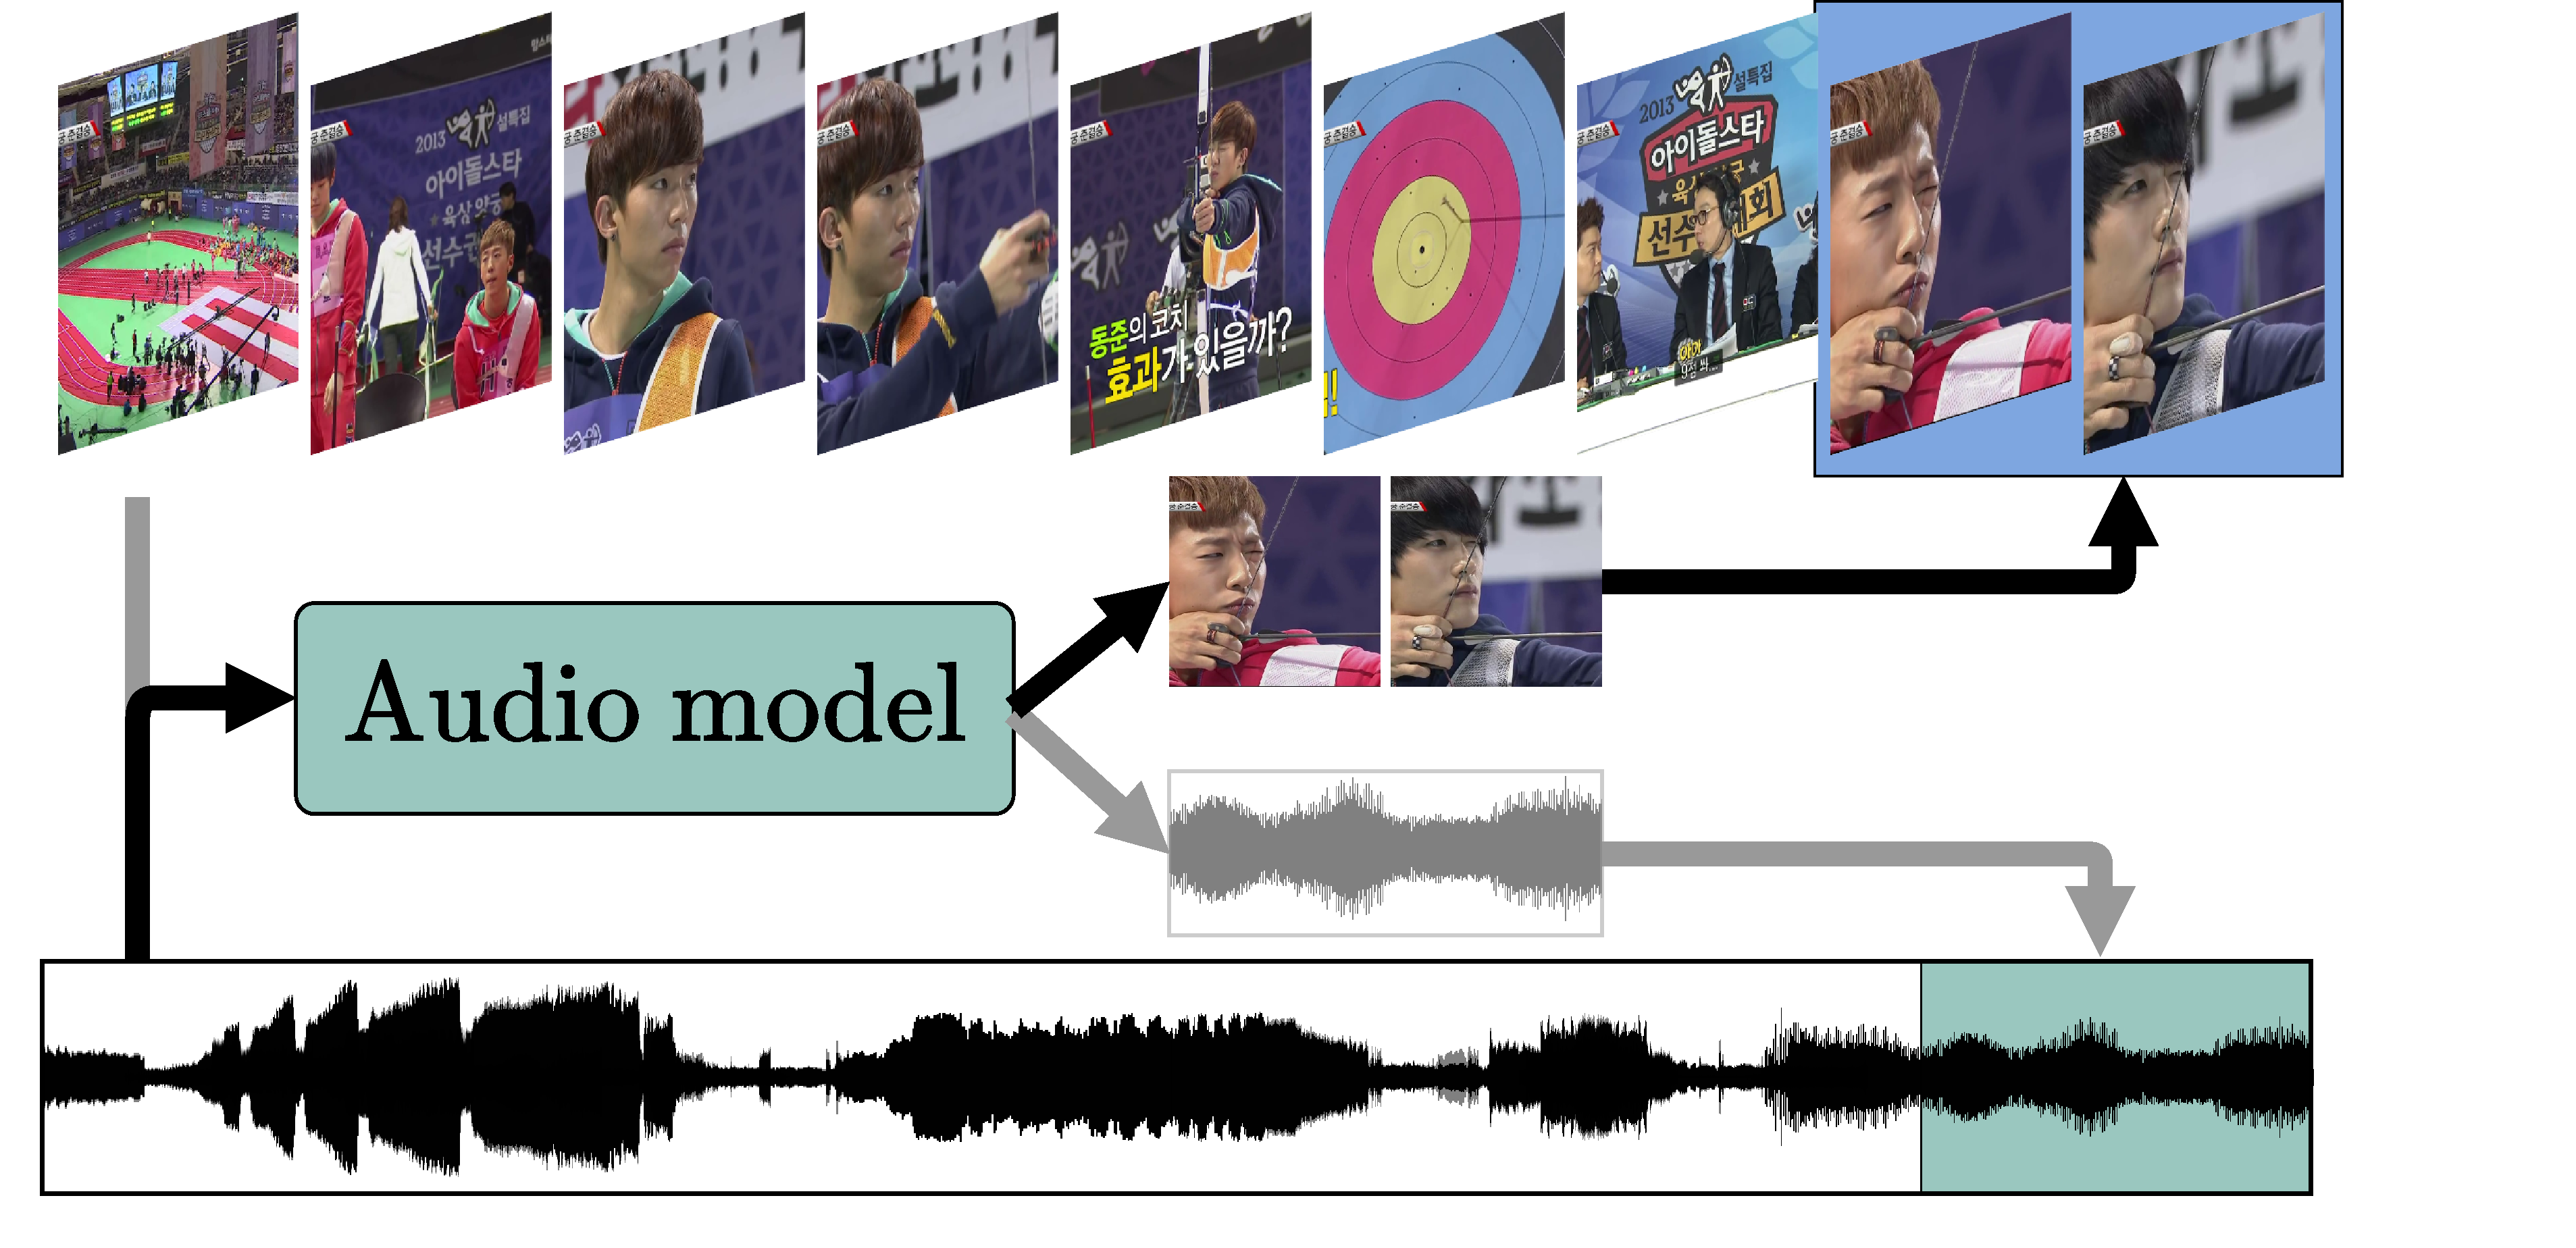
\includegraphics[width=\linewidth]{figs/redundancies_reduction/redudancies_preview.pdf}
         \caption{\textbf{Audio previewing}}
         \label{fig:redundancies_reduction::preview}
     \end{subfigure}
     \\
     \begin{subfigure}[b]{0.49\linewidth}
         \centering
         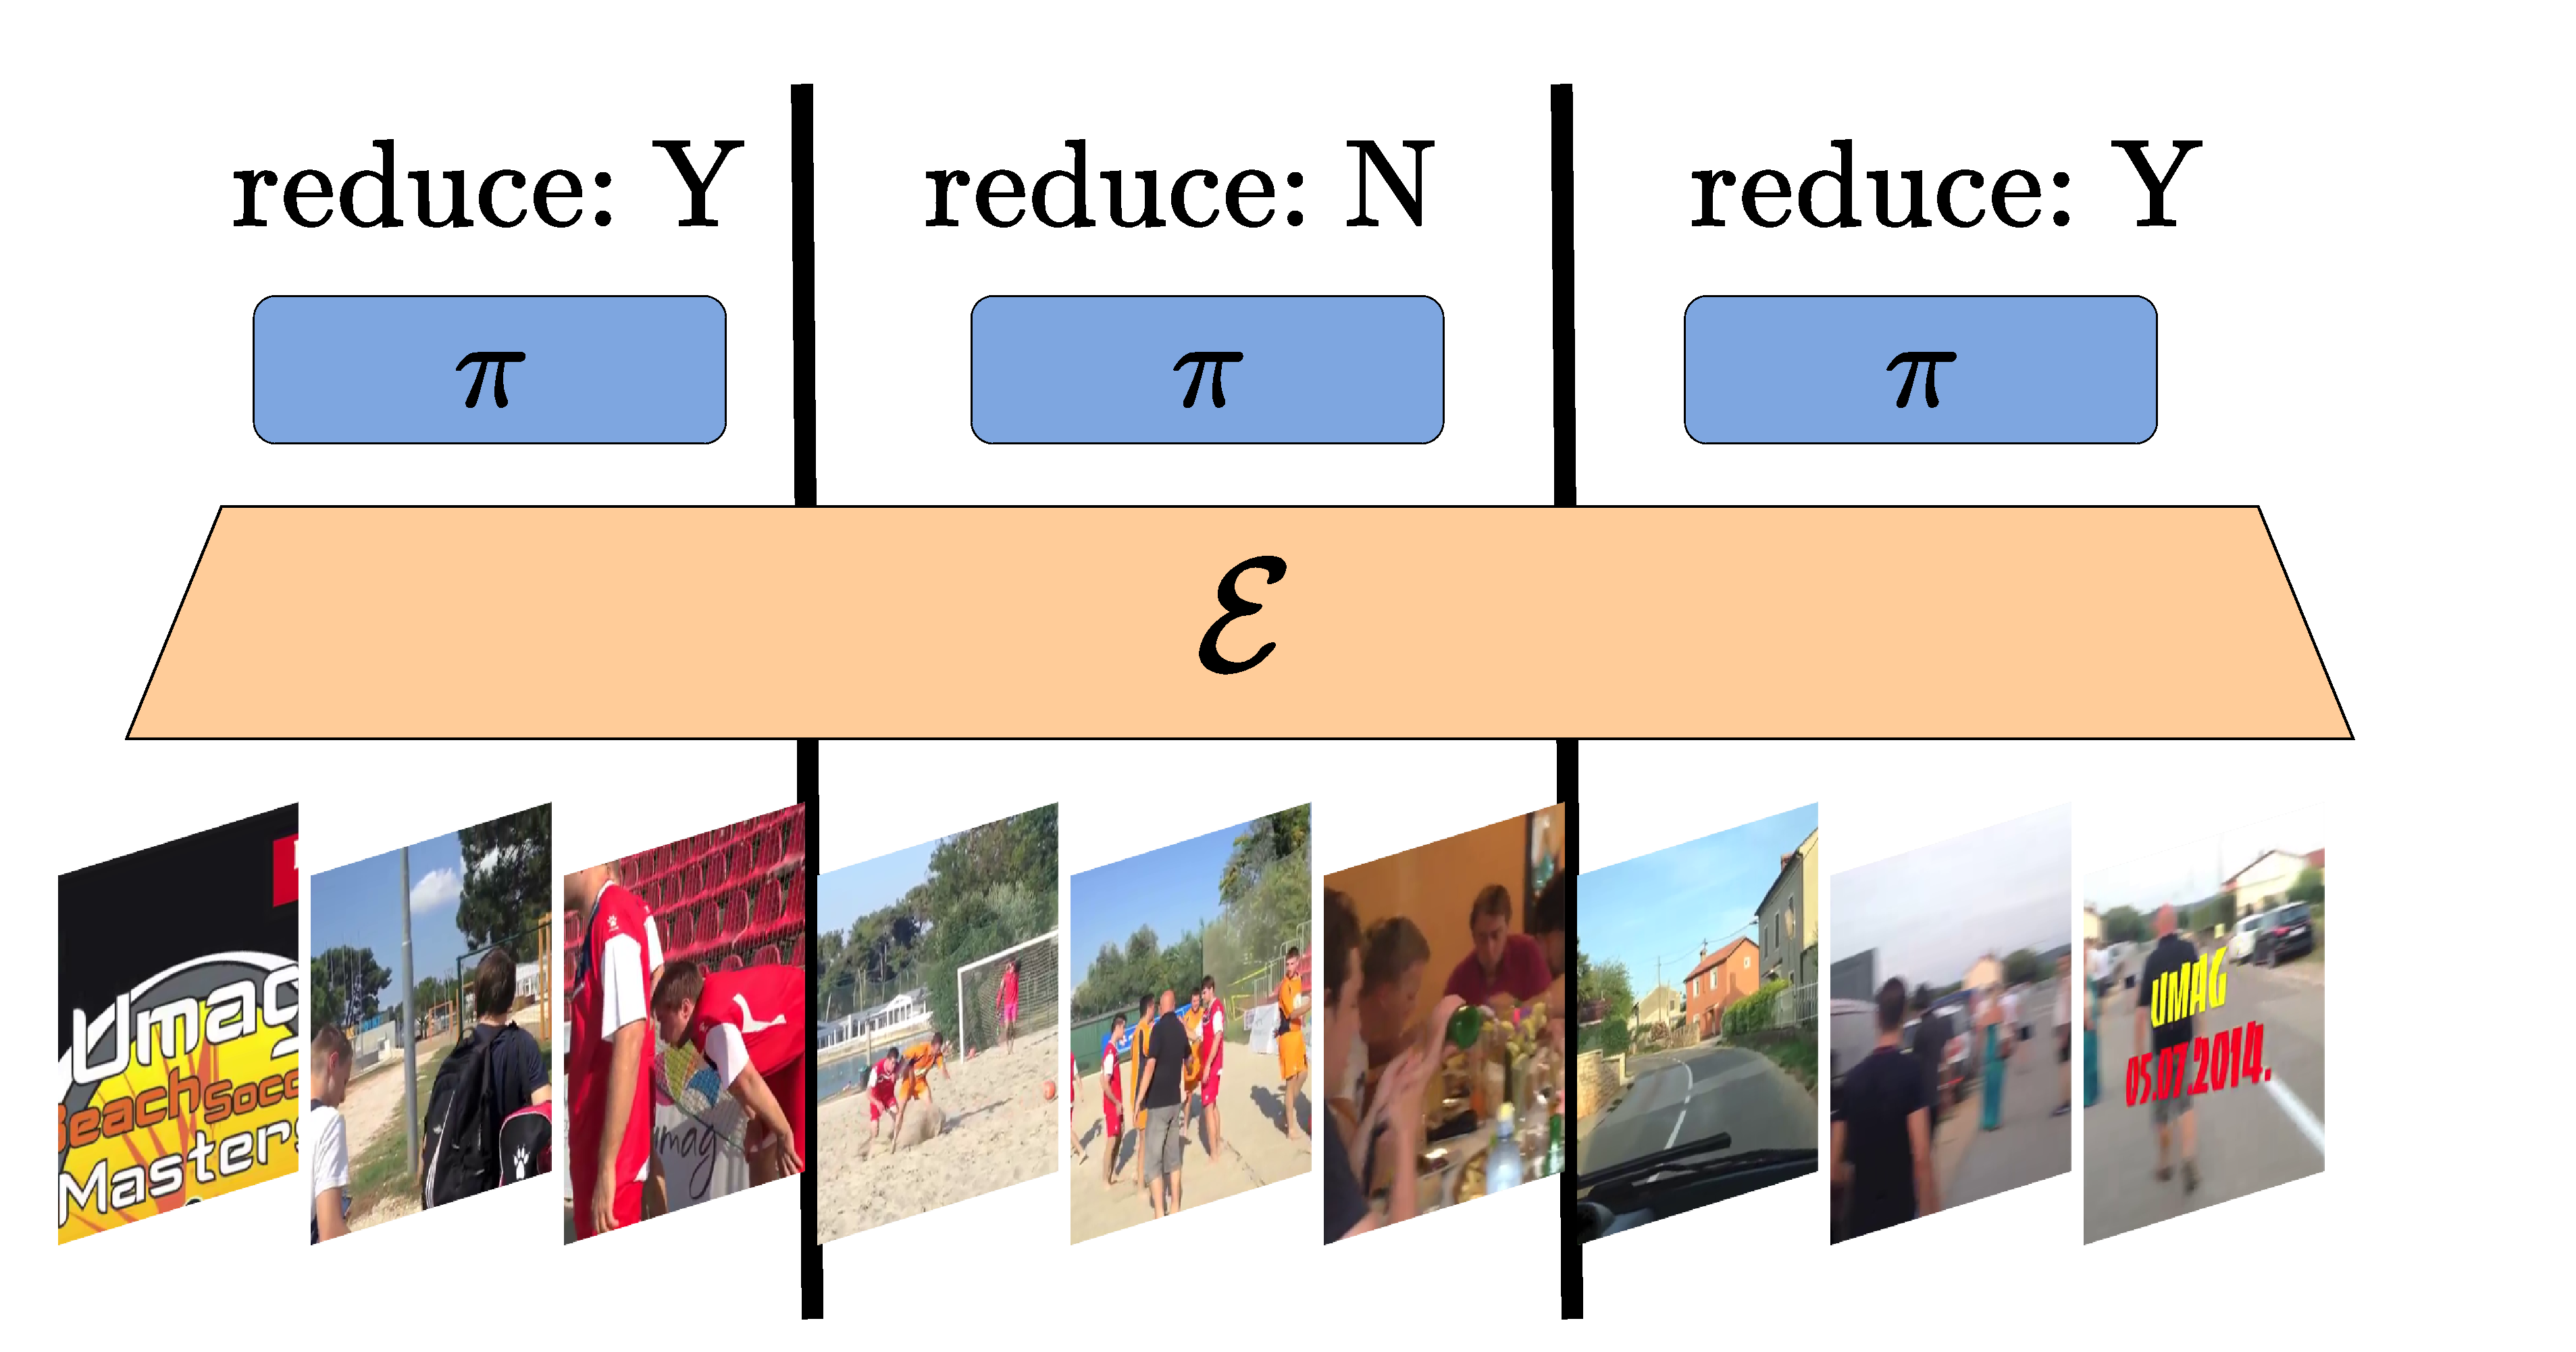
\includegraphics[width=\linewidth]{figs/redundancies_reduction/redudancies_permute.pdf}
         \caption{\textbf{Video input permuting}}
         \label{fig:redundancies_reduction::permute}
     \end{subfigure}
     \hfill
     \begin{subfigure}[b]{0.49\linewidth}
         \centering
         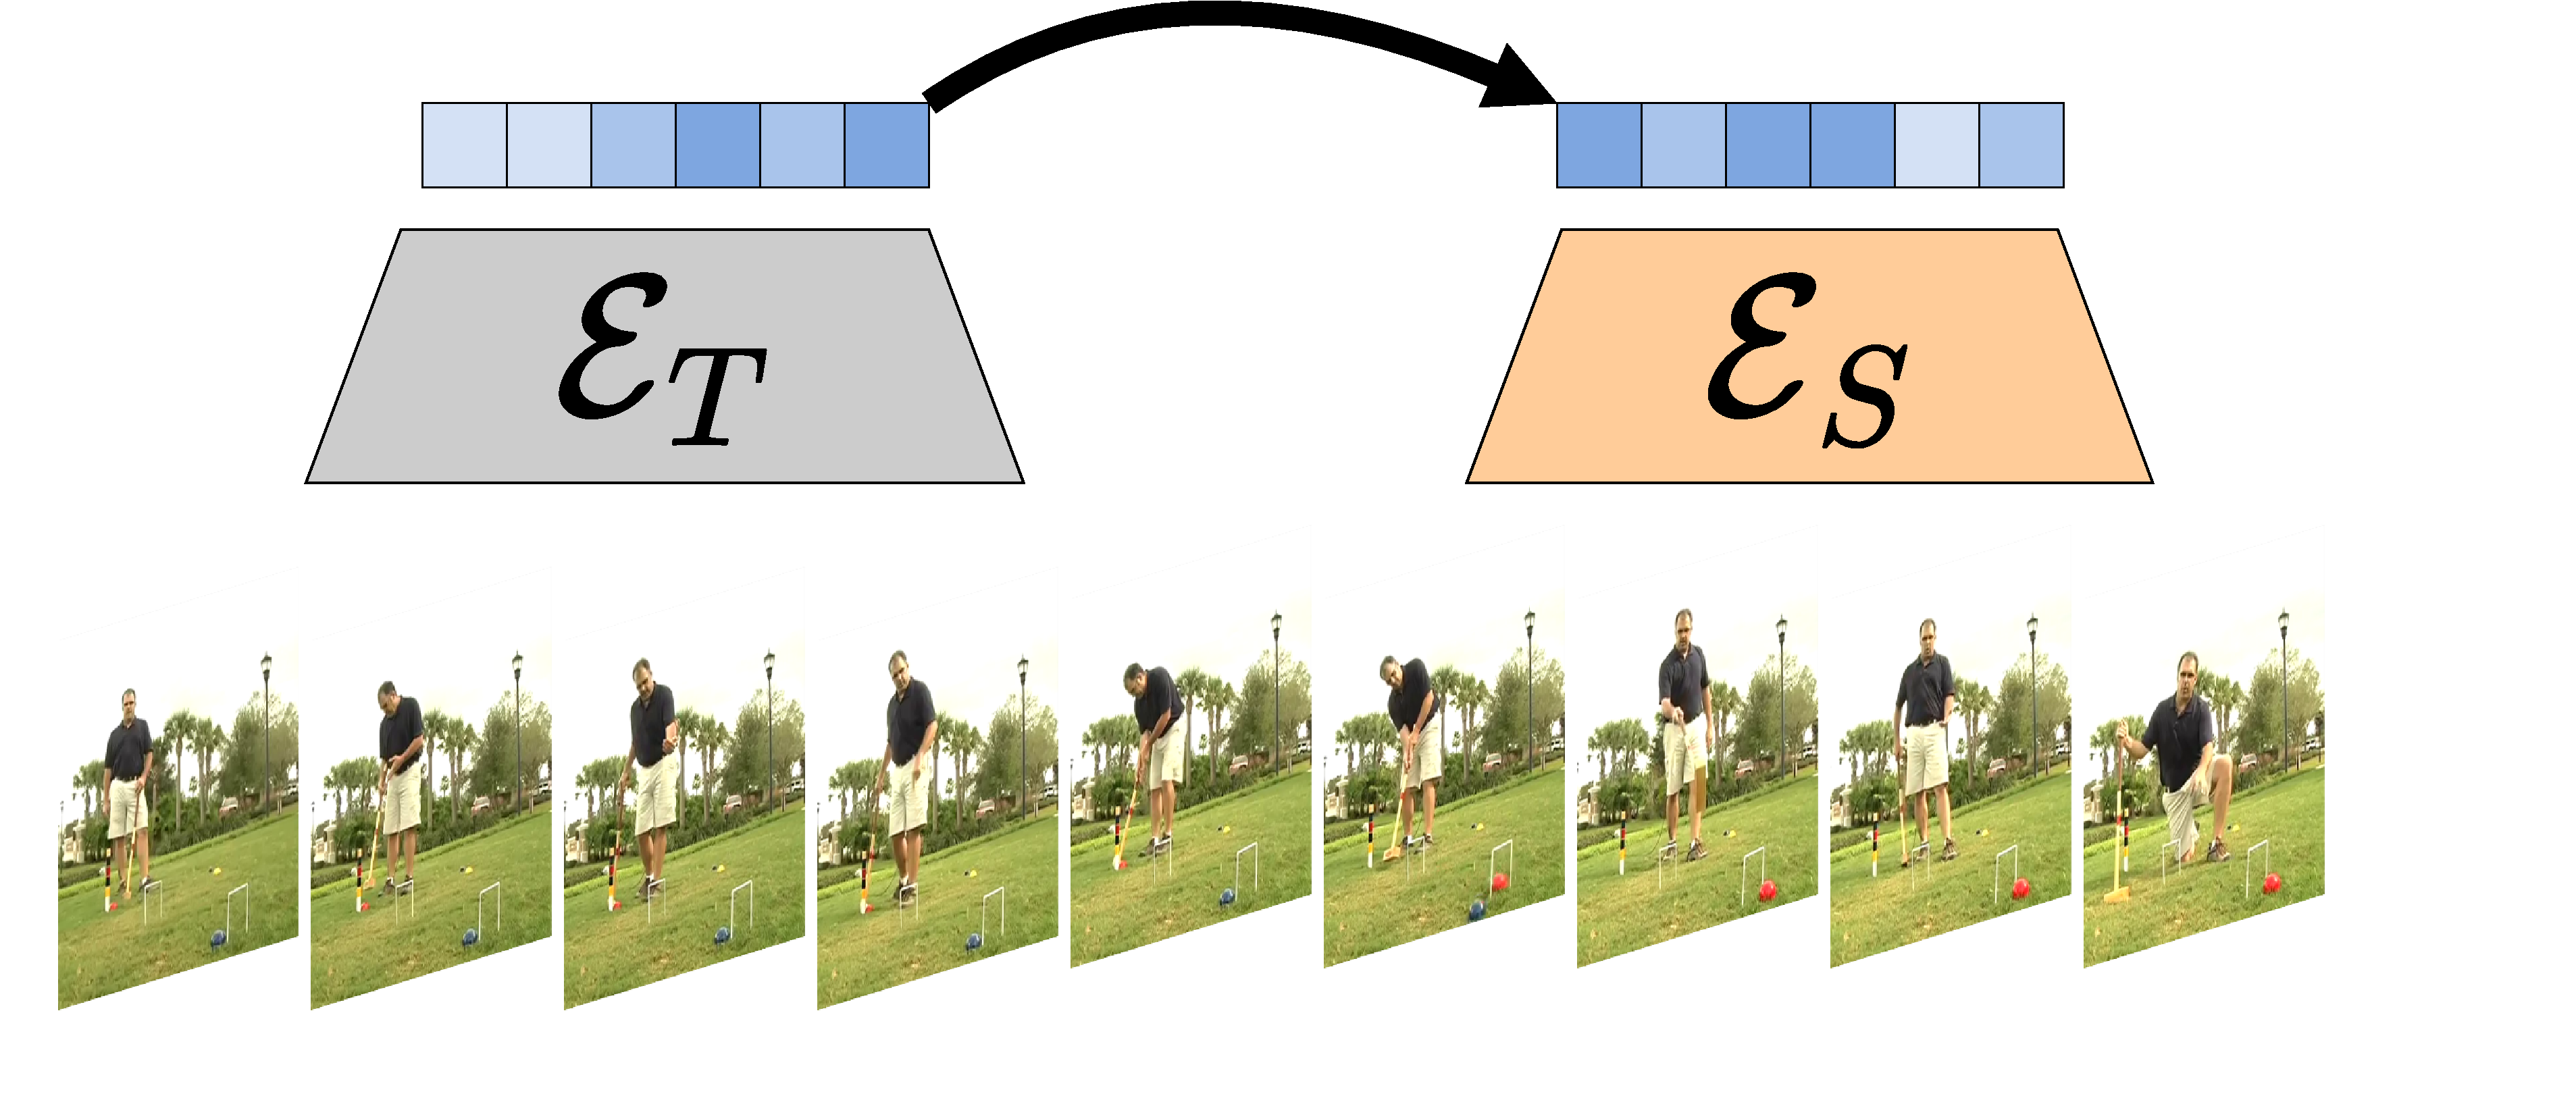
\includegraphics[width=\linewidth]{figs/redundancies_reduction/redudancies_transfer.pdf}
         \caption{\textbf{Knowledge transfer}}
         \label{fig:redundancies_reduction::transfer}
     \end{subfigure}
        \caption{\textbf{Redundancy reduction methods} include (a) selection of task-specific salient frames, (b) use of supplementary modalities such as audio to preview relevant regions to sample from, (c) input permutations to compress irrelevant frames and segments, and (d) using embeddings from a teacher model as targets.}
        \label{fig:redundancies_reduction}
\end{figure}


% ALEX: HERE

\subsubsection{Approaches}

% Frame sampling
Among the most common approaches for reducing redundancies is \emph{frame sampling}. Works on frame sampling rely on policy networks that select frames based on the action's complexity \citep{ghodrati2021frameexit,yeung2016end}, video context correspondence \citep{wu2019adaframe}, or changes in the target class' probability \citep{korbar2019scsampler}. \citet{wang2021adaptive} used a recurrent network to localize the action-relevant regions. Subsequent extensions targeted early stopping \citep{wang2022adafocus} and used features from the entire video to determine the action-relevant patches \citep{wang2022adafocusv3}. \citet{xia2022nsnet} used pseudo labels obtained by computing the embedding distance to class centroids to classify individual frames as salient and non-salient. Other approaches have used reward functions based on predictions from the selected frames \citep{wu2020dynamic}, combined frame-level and video-level predictions \citep{gowda2021smart}, optimized towards balancing accuracy and number of frames used \citep{wu2019liteeval}, or removed tokens in transformer architectures \citep{wu2024haltingvt}. %Although frame sampling can reduce input sizes, the distinction between action-relevant and irrelevant frames can lead to the loss of background context information. 

% Sampling by using an additional low-cost signal
A related set of approaches has extended unimodal frame sampling with \emph{audio previewing}. \citet{gao2020listen} used both frame and audio features with a recurrent network to predict the next informative moment in the video. The video resolution used by the model was determined based on discovered informative parts in the audio stream. Similarly, \citet{nugroho2023audio} used a saliency loss to localize the informative audio segments from which the corresponding video frames can be sampled. 

% Permuting the input (w/o sampling) to improve efficiency
Frame sampling can be beneficial in short videos. However, selecting a limited number of frames can result in information loss in longer videos with broader context. Another line of research thus studies redundancy reduction through \emph{video input permutations}. These works change frame resolutions based on classifier confidence \citep{meng2020ar} or quantize frames at different precision \citep{abati2023resq,sun2021dynamic}. \citet{zhang2022look} used a two-branch approach for lightweight computations over large, less-relevant segments, and assigned more compute for segments with relevant context similar to \citep{feichtenhofer2019slowfast}.  

% Using teacher model embeddings
Recent efforts have also used \emph{knowledge distillation} to improve the training efficiency of video model pipelines. \citet{ma2022rethinking} reduced computations by learning to match student network features from videos with reduced resolution to full resolution features from a teacher network. \citet{kim2021efficient} extended this approach by using cross-attention to learn the correspondence between teacher and student features. Distillation approaches have also used non-vision teacher models. \citet{lei2021less} bound language embeddings to sparsely sampled clips from long videos while \citet{xia2022temporal} used embeddings from textual event-object relations to discover salient frames. \citet{tan2023egodistill} proposed a reconstruction approach for interpolating egocentric video features using embeddings from partial frames and the camera motion for the unobserved frames.

\subsubsection{Future outlooks} 

Context-aware models can significantly improve both processing times and performance. Although most video reduction methods primarily evaluate their approach on classification or detection, more recent action understanding models have been optimized on multi-task and multi-domain objectives. This makes the discovery of relevant frames more difficult. For example, suppressing background frames is sub-optimal for episodic memory in which specific locations or attributes of objects not directly relevant to a current action need to be inferred. We expect that future redundancy reduction methods will focus more on preserving general scene information rather than ensuring that the semantics of objects in the scene are not lost. This can be potentially achieved by discovering informative frames for a diverse set of tasks or the distillation of scene context in low-memory representations, \eg as language embeddings.      


\begin{figure*}[t]
    \centering
    \begin{overpic}[width=\linewidth, trim={0 17cm 0 5cm},clip]{figs/localization_detection_counting.pdf}
    \put (15,0) {(a) TAL}
    \put (43,0) {(b) STAD}
    \put (71,0) {(c) VRC}
    
    \end{overpic}
    \caption{\textbf{Visualization of Temporal Action Localization (TAL), Spatio-Temporal Action Detection (STAD), Video Repetition Counting (VRC)}. TAL (a) discovers the start and end times of individual actions. In contrast, STAD (b) is more complex as it requires temporally and spatially localizing actions with bounding boxes for actors and objects over time. Distinctively, VRC (c) is not based on action labels and instead requires counting repetitions of actions or motions in an open-set setting. Video source from \citep{kay2017kinetics}.}
    \label{fig:loc_det_count}
\end{figure*}


\subsection{Temporal-based tasks}
\label{sec:recognition::temporal}

Inferring temporal information from videos is a core objective of many action recognition tasks. The perception of actions across time is a complex capability of human cognition. Understanding the timing of events is crucial for developing motor memory \citep{eagleman2010does} for actions such as moving, speaking, and determining causality of perceived temporal patterns. %Interval-, duration-, or complex temporal-combination-sensitive neural cells can temporally process events and produce timed motor responses. In parallel to human cognition, 
The importance of efficient temporal information processing in computer vision systems has been shown with both standard performance metrics and semantic benchmarks \citep{albanie2020end,stergiou2023leaping}. We provide a visualization of temporal-based tasks in \Cref{fig:loc_det_count} with the main challenges and task details discussed below.

% Main challenges in AR
\subsubsection{Challenges} 
For most tasks, action categories are inferred directly without an explicit notion of their complexity based on \textbf{levels of abstraction}, \eg, atomic movements, composite motions, singular actions, or general activities. Although some datasets include action hierarchies \citep{shao2020finegym,li2018resound}, these relationships are only used by a handful of existing works \citep{mettes2020searching}. Different levels of abstraction typically have different temporal ranges, which requires different approaches to process the visual input. Moreover, temporal variations within a class can be substantial, especially for activities. For the latter, information that can reveal the activity class can be temporally distant, requiring proper extraction and modeling of long-range dependencies. We discuss solutions to cope with these variations in this section.

% TAL definition and early works
\subsubsection{Temporal localization} 

A well-established video task is the discovery and classification of temporal segments and actions performed. Temporal Action Localization (TAL) aims to infer the action categories alongside the start and ends of the corresponding locations in untrimmed videos. 

%\noindent
%\textbf{Formulation}. Given a video $\mathbf{v}$ containing $N$ action instances of class categories $y_i \; \forall \; i \in \{1,\dots, N \}$ each with temporal boundaries $\phi_i = (\psi_i,\xi_i)$, the primary objective TAL model $f$ will minimize can be expressed as the combination of a classification $\underset{cls}{\mathcal{L}}$ and location-based regression $\underset{reg}{\mathcal{L}}$ objective.

%\begin{equation}
%    \underset{TAL}{\mathcal{L}}(f(\mathbf{v}),y_i,\phi_i) = \underset{cls}{\mathcal{L}}(\widehat{y}_i,y_i) + \underset{reg}{\mathcal{L}}(\widehat{\phi}_i,\phi_i)
%\label{eq:TAL}
%\end{equation}

%\noindent
%where $f(\mathbf{v}) = (\widehat{y}_j,\widehat{\phi}_j)$ are the $j \! \in \! \{1,\dots,\widehat{N} \}$ predicted class label $\widehat{y}_j$ and $\widehat{\phi}_j$ location  for the $\widehat{N}$ predicted classes. 

Early attempts have used Improved Dense Trajectories \citep{wang2013action} and Fisher vectors \citep{oneata2013action} to model the temporal dynamics of local points in scenes. \citet{shou2016temporal} was one of the first to approach TAL with a joint action proposal and classification objective to optimize a regional CNN. This joint optimization has been adapted in subsequent works to use spatial and temporal-only networks \citep{lin2018bsn,paul2018w,wang2017untrimmednets}, regional proposal selection \citep{chao2018rethinking,xu2017r}, and intra-proposal relationships with graph convolutions \citep{zeng2019graph}. \citet{shou2017cdc} predicted granularities at a frame level by transposing the temporal resolution of pre-trained video encoders. More recent approaches for TAL can be categorized into three broad categories. 

% Single-stage approaches
\noindent
\textbf{One-stage}. Most similar to the aforementioned methods, one-stage approaches localize and classify actions in a single step using hierarchical embeddings from feature pyramids \citep{lin2021learning,liu2020progressive,shi2023tridet,zhang2022actionformer} or discovering segments by relating relevant videos \citep{shou2018autoloc,yang2020localizing}. Recently, \citet{yan2023unloc} have explored the inclusion of vision-language encoders using the scene's semantic context for TAL. The definition of specific start and end frames of an action can lead to ambiguities. A set of approaches have relaxed their objectives to weigh the training loss by the importance of each frame within the action segment \citep{shao2023action} or by
learning distributions of possible start and end times \citep{moltisanti2019action}, putting a prior on the typical duration of the action. 

% Two-stage approaches
\noindent
\textbf{Two-stage}. Another group of methods uses an additional step to regress temporal boundaries. Two-stage approaches disentangle the optimization into separate parts. \citet{zhai2020two} combined proposals from spatial- and temporal-only streams into a fused final prediction. \citet{chen2022dcan} used long- and short-range temporal information to refine the confidence of the generated action proposals. \citet{huang2019decoupling} decoupled classification and localization to two objectives during training with two separate models that use cross-modal connections for exchanging information. Some works have focused on maximizing the embedding difference between representations of frames from action segments and non-relevant frames either with positive and negative instances \citep{luo2020weakly,zhang2021cola} or by a scoring function \citep{rizve2023pivotal}. Methods have also improved the features of backbone encoders with TAL-relevant pretext tasks \citep{zhang2022unsupervised}. A number of two-stage methods process videos holistically \citep{alwassel2021tsp,he2022asm,liu2021weakly,qing2021temporal}. \citet{alwassel2021tsp} encoded local features over a sliding window using aggregated features from multiple local encoders with a dual objective of discovering regions of actions and classifying every segment. Graphs have also been adopted for TAL with \citet{bai2020boundary} using generated candidate proposals for the graph's start and end edges and their connected nodes. \citet{zhao2021video} created a graph of hierarchical features over multiple temporal resolutions. More recent approaches \citep{nag2023difftad} have formulated proposal prediction as a denoising task with noisy action proposals as input to a diffusion model conditioned on the video. Recent approaches have also used pre-trained LLMs for TAL with specific CLIP query embeddings \citep{ju2022prompting}, video representation masks adapted to the CLIP text encoder space \citep{nag2022zero}, and CLIP text and visual features that are correlated to foreground masks learned from the video \citep{phan2024zeetad}.

% Encoder-decoder/DETR
\noindent
\textbf{DEtection TRansformers (DETR)}. A recent set of methods is based on adapting image-based DETR \citep{carion2020end} to TAL. These approaches rely on transformer encoder-decoders to create regional proposals that are optimized with bipartite matching. \citet{tan2021relaxed} adapted DETR to video with a matching scheme of multiple positive action proposals to address sparsity in temporal annotations. Subsequent works have optimized the detection pipeline by either including dense residual connections \citep{zhao2023re2tal} or caching short-term features \citep{cheng2022tallformer,hong2022spotting}. 
\citet{liu2024end} increased the model capacity by training intermediate adaptors to propagate information to the decoder from intermediate frozen encoder layers. Approaches have also explored training recipes with sparsely updating model layers \citep{cheng2022stochastic}, vision-language pre-training distillation \citep{ju2023distilling}, proposal hierarchies \citep{wu2023newsnet},
and end-to-end TAL encoder-decoder optimization \citep{liu2022empirical}. Approaches that reduce the training requirements further have been based on language embeddings with tuned visual-language projectors \citep{liberatori2024test} and by start/end queries \citep{aklilu2024zero}.



\subsubsection{Spatiotemporal detection} 

SpatioTemporal Action Detection (STAD) is related to TAL but aims to jointly localize actions temporally and spatially detect action-relevant actors and objects over frames. The main challenge of STAD methods is the consistent linking of per-frame detections and temporal action proposals. Similar to TAL, two general directions can be used to overview relevant literature. 

%\noindent
%\textbf{Formulation}. From two consecutive video $\mathbf{v}$ frames $(t,t+1)$, bounding boxes are defined as $b_t$ and $b_{t+1}$ for class $y_t$. STAD model $f$ predicts $i \in \{1,\dots,P\}$ proposals $p^i_t$ with $\widehat{y}^i_t$ label and is optimized jointly:

%\begin{gather}
%\underset{STAD \hfill}{\mathcal{L}(f(\mathbf{v}_t),y^i_t,b_t,b_{t+1})} \! = \! \underset{cls}{\mathcal{L}}(y_t,\widehat{y}^i_t) \! + \! \underset{reg}{\mathcal{L}}(p_t^i,b_t,b_{t+1})
%\label{eq:STAD}
%\end{gather}

%\noindent
%where in the regression objective $\underset{reg}{\mathcal{L}}$, proposal $p_t^i$ should be drawn closer to the ground truth bounding box of the current frame $b_t$ and the following frame $b_{t+1}$ to ensure temporal continuity.
%Similar to TAL, two general directions can be used to overview relevant literature. 

\noindent
\textbf{Two stages}. Building upon the advancements of image-based object detectors \citep{girshick2014rich,girshick2015fast}, the majority of STAD approaches first detect objects and then temporally localize actions by tracking object candidates~\citep{jain2014action,weinzaepfel2015learning}, ROI-pooling RGB and flow features \citep{peng2016multi}, iteratively refining proposals \citep{soomro2015action}, aligning source and target domain features~\citep{agarwal2020unsupervised}, or using the general action level in the video as context \citep{mettes2016spot}. \citet{li2018recurrent} build upon prior two-stage detection works with the incorporation of recurrent proposals to include temporal context. Other approaches that focus on temporal information \citet{singh2017online} use the arrow of time with different portions of the video detected at each step. Later benchmarks included longer videos to focus on activity-related tasks \citep{gu2018ava}. These have enabled the inclusion of context with feature banks \citep{feng2021relation,pan2021actor,tang2020asynchronous,wang2018videos,wu2019long,wu2022memvit} or supplementary object information \citep{arnab2021unified,hou2017tube,zhang2019structured}. Additional information such as keyframe saliency maps~\citep{li2020actions,ulutan2020actor}, hands and poses~\citep{faure2023holistic}, actor-object relations~\citep{sun2018actor}, and SSL~\citep{wang2023videomae} have also been explored. \citet{alwassel2018diagnosing} analyzed the benefits of two-stage approaches beyond performance metrics and showed that methods are primarily performant in handling temporal context. However, they also note that a significant limitation of two-stage approaches is that features are computed from backbones trained over auxiliary video tasks, potentially missing specific discriminative information.




\noindent
\textbf{Single-stage}. Drawing inspiration from single-stage object detection methods~\citep{carion2020end,redmon2016you,liu2016ssd}, single-stage STAD approaches use an end-to-end trained unified framework for joint localization and detection~\citep{chen2021watch,girdhar2019video,zhu2024dual}. \citet{ntinou2024multiscale} extended the bipartite matching loss from \citet{carion2020end} to spatio-temporal tokens. Other approaches used adaptive feature sampling~\citep{wu2023stmixer}, conditioning modeled visual features based on motion~\citep{zhao2019dance}, or contrasted different views~\citep{kumar2022end}. Directly predicting tubelets has also been adopted by recent approaches~\citep{gritsenko2024end,kalogeiton2017action,song2019tacnet,yang2019step,zhao2022tuber}. \citet{kalogeiton2017action} stacked embeddings from a backbone applied over a sliding window and regressed to both classes and tubelets over the entire video. \citet{zhao2022tuber} used an encoder-decoder to generate tubelet queries and cross-attended them to visual features. \citet{gritsenko2024end} generated candidate tubelets based on a condensed query representation that was cross-attended with features at each frame. Beyond STAD, tubelets have also been used as a self-similarity pre-training objective~\citep{thoker2023tubelet} to enforce correspondence of videos from different domains but with similar local motions. 

\subsubsection{Repetition counting}

Video Repetition Counting (VRC) is specifically aimed at counting the number of action repetitions. In contrast to TAL and STAD, VRC is an open-set task and does not require action categories.

%\noindent
%\textbf{Formulation}. Video $\mathbf{v}$ contains $C$ repetitions. VRC model $f$ can use a distance or classification-based objective to optimize repetition predictions $\widehat{c}$. If timestamps of repetitions $t \in \{1,\dots,T\}$ are available, $f$ can also use a reconstruction objective.

%\begin{gather}
%    \underset{VRC}{\mathcal{L}}(f(\mathbf{v}),\mathbf{d},c) = 
%    \begin{cases}
%    \underset{rec}{\mathcal{L}}(\widehat{\mathbf{d}},\mathbf{d}), \text{if rec-based}\\
%    \underset{dist}{\mathcal{L}}(\widehat{c},c), \text{if dist-based}\\
%    \underset{cls}{\mathcal{L}}(\widehat{c},c), \text{if cls-based}
%    \end{cases}
%\end{gather}

%\noindent
%where $\mathbf{d}$ are the density maps based on the temporal resolution of $\mathbf{v}$, the number of repetitions $c$, and each timestamp $t$. Similarly, $\widehat{\mathbf{d}}$ is the predicted density map.




\newcolumntype{g}{>{\columncolor{LightGrey}}l}

\begin{table*}[t]
    \centering
    \caption{\textbf{SSL methods and video task adaptations}. Three learning paradigms %based on context/masking/contrast
    are used to group pre-text tasks.
    %The pretext tasks are based on popularity as inspiration for video-based adaptations.
    }
    \resizebox{\linewidth}{!}{
    \setlength\tabcolsep{1.0pt}
    \begin{tabular}{c l l c l l }
    \toprule
      Learning & & Task & & Method & Video adaptations~$\textcolor{red}{^1}$  \\
      \midrule
      \multirow{5}{*}{Context-based} & \multirow{5}{*}{       
    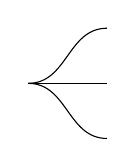
\begin{tikzpicture}
    \draw    (0,.5) .. controls (.5,.5) and (.5,1.2) .. (1,1.2) ;
    \draw    (0,.5) .. controls (.5,.5) and (.5,-.2) .. (1,-.2) ;
    \draw    (0,.5) -- (1,.5) ;
    \end{tikzpicture}
      }&  Arrow of Time & & & \makecell[l]{
      \citet{benaim2020speednet},
      \citet{dwibedi2018temporal},
      \citet{destro2024cyclecl},
      \citet{donahue2024learning}, \\
      \citet{salehi2023time},
      \citet{wei2018learning},
      \citet{wu2021contrastive}
      }  \tstrut \bstrut \\
      & & \multicolumn{1}{g}{Jigsaw} & \multicolumn{1}{g}{} & \multicolumn{1}{g}{} & \multicolumn{1}{g}{\tabularCenterstack{l}{
      \citet{kim2019self},
      \citet{lee2017unsupervised},
      \citet{liu2024solving},
      \citet{misra2016shuffle},
      \citet{wang2022video}, \\
      \citet{xu2019self}
      }} \tstrut \bstrut \\
      & & Colorization & & & \makecell[l]{
      \citet{ali2023task},
      \citet{dhiman2023corf},
      \citet{jabri2020space},
      \citet{liu2024temporally},
      \citet{vondrick2018tracking},\\
      \citet{wu2020memory},
      \citet{zhang2023temporal}
      } \tstrut \bstrut \\
      \multirow{16}{*}{Contrastive} & \multirow{16}{*}{       
    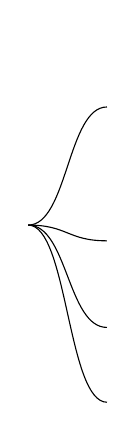
\begin{tikzpicture}
    \draw (0,3) -- (0,3);
    \draw (0,0) -- (0,0);
    \draw    (0,0.5) .. controls (.5,0.5) and (.5,2.) .. (1,2.) ;
    \draw    (0,.5) .. controls (.5,0.5) and (.5,.3) .. (1,.3) ;
    \draw    (0,.5) .. controls (.5,.5) and (.5,-.8) .. (1,-.8) ;
    \draw    (0,.5) .. controls (.5,.5) and (.5,-1.75) .. (1,-1.75) ;
    \end{tikzpicture}
      }&\multirow{8}{*}{Negative Samples} & \multirow{8}{*}{       
    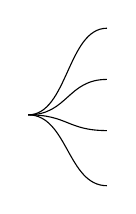
\begin{tikzpicture}
    \draw    (0,-.1) .. controls (.5,-.1) and (.5,1) .. (1,1) ;
    \draw    (0,-.1) .. controls (.5,-.1) and (.5,.35) .. (1,.35) ;
    \draw    (0,-.1) .. controls (.5,-.1) and (.5,-.3) .. (1,-.3) ;
    \draw    (0,-.1) .. controls (.5,-.1) and (.5,-1) .. (1,-1) ;
    \end{tikzpicture}
      } & \multicolumn{1}{g}{MoCo \citep{he2020momentum}} & \multicolumn{1}{g}{\tabularCenterstack{l}{
      \citet{feichtenhofer2021large},
      \citet{han2020memory},
      \citet{kuang2021video}, 
      \citet{liu2021hit},\\
      \citet{ma2021active},
      \citet{pan2021videomoco},
      \citet{qian2021spatiotemporal},
      \citet{xu2021rethinking},
      \citet{yao2021seco} }} \tstrut \bstrut \\
      && && SimCLR \citep{chen2020simple} & \makecell[l]{
      \citet{badamdorj2022contrastive},
      \citet{chen2021rspnet},
      \citet{han2020self},
      \citet{jenni2021time}, \\
      \citet{sun2021composable},
      \citet{wang2020self},
      \citet{yang2020video},
      \citet{zhang2021video}
      } \tstrut \bstrut \\
      && && \multicolumn{1}{g}{CPC \citep{oord2018representation}} & \multicolumn{1}{g}{\tabularCenterstack{l}{
      \citet{akbari2021vatt},
      \citet{bagad2023test}
      \citet{dave2022tclr},
      \citet{li2021motion},
      \citet{miech2020end}, \\
      \citet{park2022probabilistic},
      \citet{parthasarathy2023self},
      \citet{yang2021taco}}} \tstrut \bstrut \\
      && && DIM \citep{hjelm2018learning} & \makecell[l]{
      \citet{bai2022salient},
      \citet{cai2022heterogeneous},
      \citet{feng2023mutual},
      \citet{gordon2020watching}, \\
      \citet{hjelm2020representation},
      \citet{nan2021interventional},
      \citet{sameni2023spatio},
      \citet{sun2019learning}
      } \tstrut \bstrut \\
      && Clustering & \multirow{1}{*}{ 
    \begin{tikzpicture}
    \draw (0,.5) -- (0,.5) ;
    \draw   (0,0.6) -- (1,.6) ;
    \end{tikzpicture}
      } & \multicolumn{1}{g}{SwAV \citep{caron2020unsupervised}} & \multicolumn{1}{g}{
      \tabularCenterstack{l}{
      \citet{coskun2022goca},
      \citet{diba2021vi2clr},
      \citet{long2023cross},
      \citet{toering2022self},\\
      \citet{wei2022inter},
      \citet{yan2020clusterfit}
      }
      } \\
      && \multirow{4}{*}{Self-Distillation} & \multirow{4}{*}{ 
    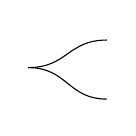
\begin{tikzpicture}
    \draw (0,0) -- (0,0) ;
    \draw   (1,1) -- (1,1) ;
    \draw    (0,.5) .. controls (.5,.5) and (.5,.85) .. (1,.85) ;
    \draw    (0,.5) .. controls (.5,.5) and (.5,.1) .. (1,.1) ;
    \end{tikzpicture}
      }& BYOL \citep{grill2020bootstrap} & \makecell[l]{
      \citet{escontrela2023video},
      \citet{liu2022funnynet},
      \citet{morales2022leveraging},
      \citet{recasens2021broaden},\\
      \citet{ranasinghe2022self},
      \citet{sarkar2023uncovering},
      \citet{xiong2021self},
      \citet{zhang2022contrastive}
      } \\
       && && \multicolumn{1}{g}{DINO \citep{caron2021emerging}} & \multicolumn{1}{g}{\tabularCenterstack{l}{
       \citet{ding2024betrayed},
       \citet{fan2023unsupervised},
       \citet{huang2024vbench},
       \citet{huang2024uvis},\\
       \citet{ponimatkin2023simple},
       \citet{teeti2023temporal},
       \citet{wang2024videocutler}
       }} \\
       && \multirow{2}{*}{Decorrelation} &\multirow{1}{*}{ 
    \begin{tikzpicture}
    \draw (0,0) -- (0,0) ;
    \draw   (1,1) -- (1,1) ;
    \draw    (0,.66) .. controls (.5,.66) and (.5,.85) .. (1,.85) ;
    \draw    (0,.66) .. controls (.5,.66) and (.5,.45) .. (1,.45) ;
    \end{tikzpicture}
      } & Barlow Twins \citep{zbontar2021barlow} & \multirow{1}{*}{
      \citet{da2022unsupervised},
      \citet{peh2024learning},
      \citet{zhang2022contrastive},
      \citet{zhou2023self}
      } \\
       && && \multicolumn{1}{g}{VICReg \citep{bardes2021vicreg}} & \multicolumn{1}{g}{
       \multirow{1}{*}{
       \citet{bardes2023mc},
       \citet{sun2023unified},
       \citet{yang2023contrastive},
       \citet{yu2024evolve}
       }
       } \\
       \multirow{7}{*}{Masking} &
       \multirow{7}{*}{       
    \begin{tikzpicture}
    \draw (0,3) -- (0,3);
    \draw (0,0) -- (0,0);
    \draw    (0,1.8) .. controls (.5,1.8) and (.5,2.7) .. (1,2.7) ;
    \draw    (0,1.8) .. controls (.5,1.8) and (.5,1.8) .. (1,1.8) ;
    \draw    (0,1.8) .. controls (.5,1.8) and (.5,1.25) .. (1,1.25) ;
    \end{tikzpicture}}
    & \multirow{2}{*}{low-level targets} & \multirow{1}{*}{ 
    \begin{tikzpicture}
    \draw (0,0) -- (0,0) ;
    \draw   (1,1) -- (1,1) ;
    \draw    (0,.66) .. controls (.5,.66) and (.5,.85) .. (1,.85) ;
    \draw    (0,.66) .. controls (.5,.66) and (.5,.45) .. (1,.45) ;
    \end{tikzpicture}
      }& ViT \citep{dosovitskiy2020image} & \makecell[l]{
      \citet{girdhar2023imagebind},
      \citet{lin2022frozen},
      \citet{piergiovanni2023rethinking}
      } \\
       && && \multicolumn{1}{g}{MAE \citep{he2022masked}} & \multicolumn{1}{g}{\tabularCenterstack{l}{
       \citet{feichtenhofer2022masked}, \citet{girdhar2023omnimae}, \citet{huang2023mgmae}, \citet{huang2023mavil}, \\ \citet{ryali2023hiera},  \citet{tong2022videomae}, \citet{wang2023videomae}, \citet{wu2023dropmae}}} \\
       && high-level targets & \multirow{1}{*}{ 
    \begin{tikzpicture}
    \draw (0,0) -- (0,0) ;
    \draw   (1,1) -- (1,1) ;
    \draw    (0,.85) .. controls (.5,.85) and (.5,.85) .. (1,.85) ;
    \end{tikzpicture}
      }& BEiT \citep{bao2021beit} & \makecell[l]{
      \citet{cheng2023vindlu},
      \citet{fu2021violet},
      \citet{li2023svitt},
      \citet{tan2021vimpac},
      \citet{wang2022bevt}
      } \\
       && \multirow{2}{*}{Teacher-based} &\multirow{1}{*}{ 
    \begin{tikzpicture}
    \draw (0,0) -- (0,0) ;
    \draw   (1,1) -- (1,1) ;
    \draw    (0,.66) .. controls (.5,.66) and (.5,.85) .. (1,.85) ;
    \draw    (0,.66) .. controls (.5,.66) and (.5,.45) .. (1,.45) ;
    \end{tikzpicture}
      }& \multicolumn{1}{g}{data2vec \citep{baevski2022data2vec}} & \multicolumn{1}{g}{
      \tabularCenterstack{l}{
      \citet{li2023unmasked},
      \citet{lian2023av}
      }
      } \\
       && && MaskFeat \citep{wei2022masked} & 
       \makecell[l]{
       \citet{feichtenhofer2022masked},
       \citet{mizrahi20234m},
       \citet{lin2023smaug},
       \citet{pei2024videomac} \\
       \citet{stergiou2024holistic}, 
       \citet{wang2023masked},
       \citet{woo2023towards},
       \citet{zhao2024asymmetric}
       }  \\
      \end{tabular}
    }
    \label{tab:SSL_tasks}
    \vspace{-1em}
\end{table*}

Early works relied on signal periodicity \citep{thangali2005periodic}, decomposing signal repetition with a Fourier analysis \citep{branzan2008generic,briassouli2007extraction,ousman2008segmentation,ross2000robust,pogalin2008visual}. Signal-based works have also used the direction of motion flow over time \citep{runia2018real} to count repetitions. Another set of methods approached VRC as a classification task over a finite set of maximum repetitions. \citet{lu2004repetitive} used dynamic parameters based on the Frobenius norm to classify changes corresponding to action end times.
\citet{zhang2021repetitive} fused audio and video representations while \citet{zhang2020context} used multiple cycles to refine the repetition count prediction. \citet{li2024efficient} extracted action query features and classified the queries for repeating actions. In contrast to defining repetition counts as classes, \citet{dwibedi2020counting} adopted a temporal self-similarity matrix \citep{benabdelkader2004gait,junejo2010view,korner2013temporal} to discover repetition periodicity. Subsequent methods have investigated embedding similarity matrices at multiple scales \citep{bacharidis2023repetition,hu2022transrac}, triplet contrastive losses \citep{destro2024cyclecl}, and graph representations \citep{panagiotakis2018unsupervised}. Because embeddings of adjacent frames are highly similar, several recent methods have aimed to limit the discovery of correspondences in repetitions to poses \citep{ferreira2021deep,yao2023poserac}, specific frames \citep{li2024repetitive,zhao2024skim}, visual exemplars \citep{sinha2024every}, or language descriptions \citep{dwibedi2024ovr}. VRC remains a challenging task given the open-set nature and the lack of robust baselines in recent large-scale datasets \citep{dwibedi2024ovr}.

\subsubsection{Future outlooks}

Despite the great progress across temporal tasks, generalizing across multiple temporal-based tasks with unified systems remains challenging. For example, STAD methods \citep{dai2021pdan,tirupattur2021modeling} benchmarked on TAL perform lower than TAL-based models as their joint objective of localizing both \emph{when} and \emph{where} actions are performed, is significantly more challenging to optimize. Similarly, despite the task similarities between TAL and VRC, standard TAL methods do not generalize to VRC as action interruptions and out-of-distribution categories cannot be effectively segmented \citep{hu2022transrac,sinha2024every}. The recent introduction of unified video-language frameworks for multiple video tasks by \citet{wang2024internvideo2} and its use as a feature extractor in subsequent works \citep{chen2024video}, has shown a promising direction through the use of SSL. The proposed training recipe includes three stages of contrastive and masking self-supervision pre-text objectives to allow the generalization of the model to multiple tasks. Training on SSL pre-text tasks is a prominent scheme for many video-based models as shown in \Cref{tab:SSL_tasks}. A possible direction of future research can be the unification of downstream objectives through relevant pre-text tasks based on the context using \emph{the arrow of time}, relationships between task-specific embeddings, or clustering embeddings of semantically similar tasks.     




\subsection{Language semantics in videos}
\label{sec:recognition::language}

%\blfootnote{$\textcolor{red}{^1}$ For better readability we maximally show the ten more relevant video adaptation methods.}
The advancements of LLMs have achieved great success in Natural Language Processing (NLP), and have consequently been adapted for action understanding tasks. The relationships between learned context-rich semantic space and visual world attributes are useful for tasks such as caption generation~\citep{seo2022end,sun2019videobert,wang2024omnivid} and inferring scene information~\citep{anderson2018vision,cheng2024egothink}, or for understanding the general context in highlight detection~\citep{lei2021detecting} and instructional video learning~\citep{miech2020end}. Beyond their direct applicability to language-based tasks, the majority of Vision-Language Models (VLMs)~\citep{ashutosh2023hiervl,fu2021violet,kahatapitiya2024victr,song2024moviechat,xu2021videoclip,zellers2021merlot} focus on training encoders of general and semantically-rich representations that can then be used as feature extractors in downstream tasks. Despite the popularity of SSL with language embeddings for distilling context into video models, notable challenges persist. 

\subsubsection{Challenges}

Visual and language information can provide partly complementary perspectives of a video. However, information from each modality is often heterogeneous, with specific representations that are not directly matched through cross-modal correspondence, \eg, due to occluded objects or fine-grained visual details about the performance of the action. Such discrepancies can be based on domain knowledge of the cross-modal connections or the distribution patterns of the available data~\citep{liang2024foundations}. \textbf{Modality gap}~\citep{liang2022mind}, shown in \Cref{fig:mod_gap}, is a common phenomenon of VLM models in which embeddings of each modality are represented in distinct low-variance regions in the embeddings space. For VLMs trained with cross-modal information maximization~\citep{bain2021frozen,lei2021less,li2020hero,li2022align,zhu2020actbert} this effect becomes stronger with the enforcement of strong coordination based on positive and negative cross-modal pairs. This is also relevant to the difficulties in the \textbf{cross-modal context alignment} over local elements for tasks with available ground-truth pairs and global representations for tasks without cross-modal pairs. In both cases, aligning language and vision context information at either the word/object level or over groups of instances in the embedding space provides a significant challenge in optimization. For generative tasks, this can also lead to difficulties in \textbf{modality specific generation}. The generation of semantic-rich data based on relationships from auxiliary modalities with ambiguous correspondence can impact approaches based on either conditional, stochastic, or auto-regressive generation.

\begin{figure}[t]
    \centering
    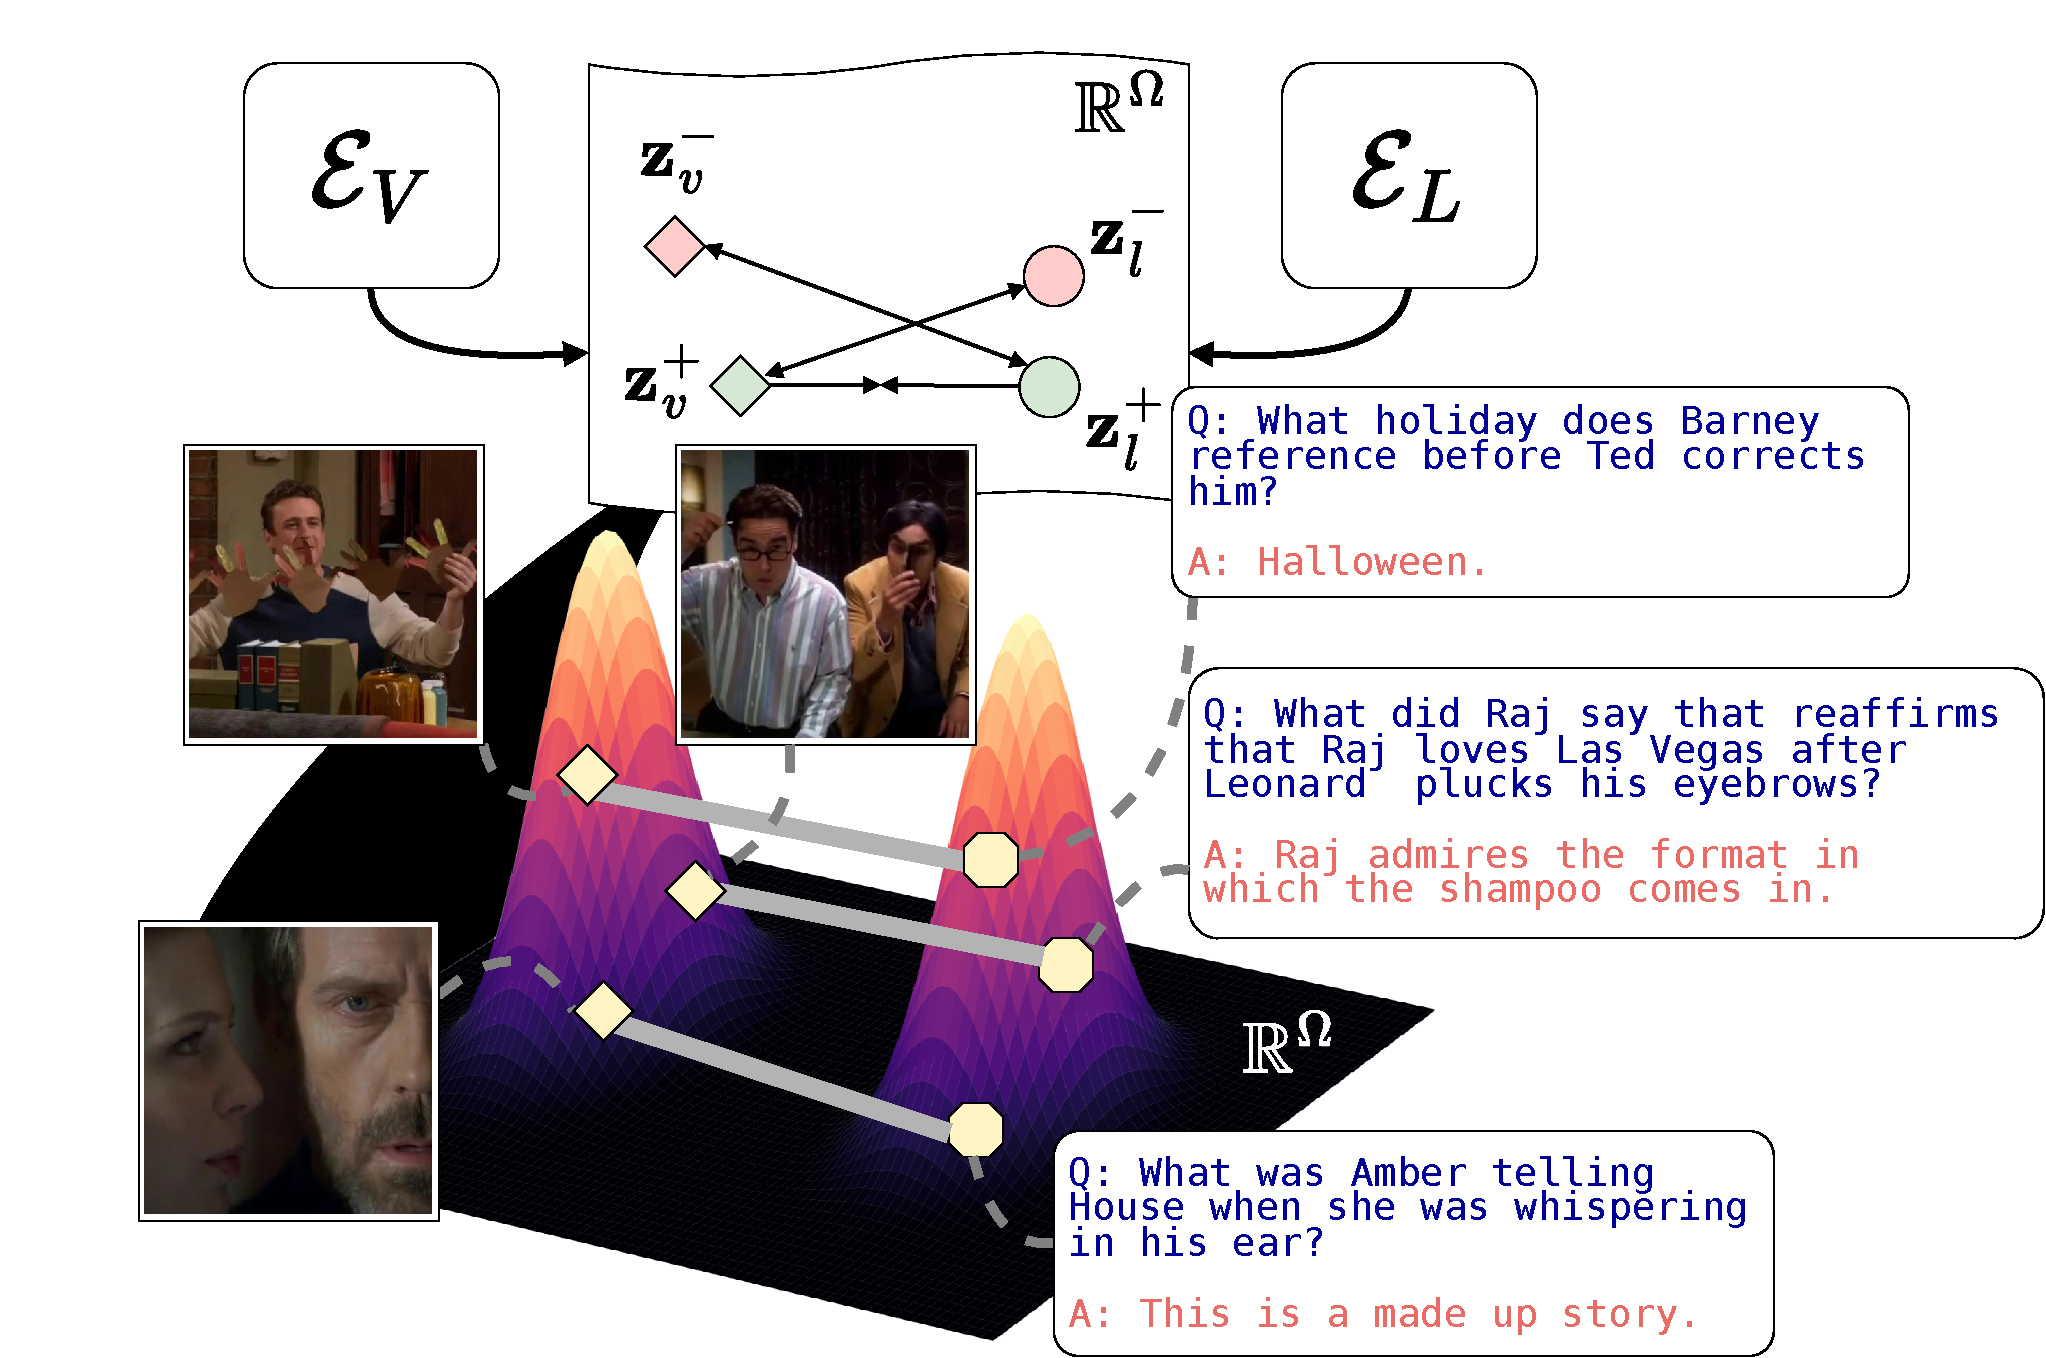
\includegraphics[width=\linewidth]{figs/mind_the_gap.pdf}
    \caption{\textbf{VLM modality gap}. Given video encoder $\mathcal{E}_V$ and text encoder $\mathcal{E}_L$, video and text are encoded to embeddings $\mathbf{z}_v^{+}$ and $\mathbf{z}_l^{+}$ in a joint embedding space $\mathbb{R}^{\Omega}$. VLM objectives align both $\mathbf{z}_v^{+}$ and $\mathbf{z}_l^{+}$. Contrastive approaches~\citep{chen2020simple,oord2018representation,xu2021videoclip} additionally maximize the distance between negative vision-language pairs: ($\mathbf{z}_v^{+}$, $\mathbf{z}_l^{-}$) and ($\mathbf{z}_v^{-}$, $\mathbf{z}_l^{+}$). Despite high-level semantic similarity, relevant modality-specific information that is not transferable across modalities can lead to a \emph{modality gap} over embeddings. Videos sourced from \citet{lei2018tvqa}.}
    \label{fig:mod_gap}
    \vspace{-1em}
\end{figure}


\begin{figure*}
    \centering
    \begin{overpic}[width=\linewidth,keepaspectratio]{figs/retreival_tasks.pdf}
        \put(2,-1){(a) \textbf{Instance-based}}
        \put(58,-1){(b) \textbf{Semantics-based}}
        \put(84,-1){(c) \textbf{TSG}}
    \end{overpic}
    \caption{\textbf{Video retrieval tasks}. Instance-based retrieval (a) returns only a single video corresponding to a search query. Semantics-based retrieval (b) returns a ranking score corresponding to each video's relevance to the search query. Temporal Sentence Grounding (TSG) (c) receives \textbf{video segments from queries} and returns the start and end time per segment.}
    \label{fig:retreival_tasks}
\end{figure*}


\subsubsection{Vision-language retrieval} 


Video retrieval sources relevant videos from a dataset based on an input query in natural language. As shown in \Cref{fig:retreival_tasks}, research works can be categorized into two groups.


\noindent
\textbf{Instance-based}. Image methods have explored cross-view ranking~\citep{wang2016learning}, language to visual attention~\citep{torabi2016learning}, or using visual features as embedding targets for language encodings~\citep{dong2018predicting}. Early adaptation of visual-language approaches to videos have used image-text-video triplets \citep{otani2016learning}, or relating parts of speech to objects and actions \citep{gabeur2020multi,xu2015jointly}. %Formally, given a set of videos $\mathbf{V}$ and a corresponding set captions $\mathbf{Y}$, instance-based approaches use a binary score function to rank correspondence:

%\begin{gather}
%    S(\mathbf{v}_i,y_j) = \mathbbm{1}(\|i-j\|=0) \; \forall \; \mathbf{v}_i \in \mathbf{V}\; \text{and} \; y_j \in \mathbf{Y}
%\label{eq:VR_inst}
%\end{gather}

In general, instance-based approaches use a binary score function to rank correspondences. Refinements to this objective have been made through visual-language binding with the inclusion of parts-of-speech in target captions \citep{wray2019fine} and dual object-text and action-text models \citep{liu2019use,mithun2018learning}. A number of methods have studied vision-language pre-training approaches \citep{ge2022bridging,lin2022egocentric,xue2022advancing}. \citet{ge2022bridging} related verbs and nouns to questions and video segments. \citet{xue2022advancing} studied the correspondences between keyframes and all video frames, subsequently contrasting the keyframe-fused video features to language embeddings.



\noindent
\textbf{Semantics-based}. A more challenging task is to retrieve images based on shared semantics to the query image~\citep{gordo2017beyond}. Semantic-based approaches primarily use triplet losses that contrastively regress between text queries and corresponding positive and negative visual inputs.
%$q$, corresponding positive visual inputs $\mathbf{x}^{+}$, and negative visual inputs $\mathbf{x}^{-}$.

%\begin{gather}
%\underset{sem}{\mathcal{L}}(q,\mathbf{x}^{+},\mathbf{x}^{-}) = \underset{t2v}{\mathcal{L}}(q,\mathbf{x}^{+},\mathbf{x}^{-}) + \underset{v2t}{\mathcal{L}}(q,\mathbf{x}^{+},\mathbf{x}^{-})
%\label{eq:VR_sem}
%\end{gather}

%\noindent
%where $\underset{t2v}{\mathcal{L}}$ and $\underset{v2t}{\mathcal{L}}$ are the losses that reduce the embeddings distance of the cross-modal pair $(q,\mathbf{x}^{+})$ together and increase distance between $(q,\mathbf{x}^{-})$.

Video retrieval works have studied this through either a contrastive objective based on a support set of videos with similar action categories \citep{patrick2020support} or a semantic
similarity scoring function for videos from the same category \citep{wray2021semantic}. Recently, \citet{kim2024you} have utilized prior knowledge in retrieving text features based on prior high embedding correspondences to similar visual features. \citet{chun2021probabilistic} created probabilistic representations of visual features to accommodate multi-query relevance. Similarly, \citet{li2023progressive} created an object-phrase and event-phrase prototype-matching framework to enforce relations between high-level concepts across modalities. \citet{hao2024uncertainty} employed an uncertainty estimate based on the Wasserstein distance between source and target domains of text-vision pairs.




\noindent
\textbf{Temporal sentence grounding (TSG)}. TSG \citep{regneri2013grounding} localizes moments in videos based on provided natural language queries. Compared to retrieving entire videos, TSG only retrieves segments from a video. The task closely relates to TAL as also shown by the number of overlapping works \citep{gao2017tall} jointly exploring the two tasks. However, in contrast to TAL, TSG requires both natural language reasoning between query and answer, and language and vision reasoning with query-video and answer-video relevance. Following \citep{gao2017tall}, a broad formulation of TSG includes a visual-language semantic alignment between video and sentence embeddings. A regression loss is used for the temporal location of the sentence.

%$\underset{aln}{\mathcal{L}}$ between video embeddings $\mathbf{z}_v$ and sentence embeddings $\mathbf{z}_l$ from model $f$. In addition a regression loss is used for the temporal location of the sentence. The final objective is defined as:

%\begin{gather}
%\underset{TSG}{\mathcal{L}}(f(\mathbf{v},t),\phi) = \underset{aln}{\mathcal{L}}(\mathbf{z}_v,\mathbf{z}_l) + \underset{reg}{\mathcal{L}}(\widehat{\phi},\phi)
%\label{eq:tsg}
%\end{gather}

%\noindent
%where $\phi$ and $\widehat{\phi}$ are the start and end times of the corresponding segment.


Early approaches have explored region proposals \citep{chen2018temporally,qu2020fine,liu2018cross}, ranking \citep{escorcia2019temporal}, distance-based joint vision-language embeddings \citep{anne2017localizing,rohrbach2016grounding}, and cross-modal graph representations \citep{liu2022memory,zhang2019man}. As
the association of visual and text features can be performed at multiple levels of abstraction, subsequent methods have learned correspondences over multiple proposals \citep{xu2019multilevel}, local and global information \citep{jiang2019cross,mun2020local}, and word/sentence-level cues \citep{hao2022query}. \citet{zhang2021natural} used language-guided highlighting by cross-attending text features to multi-resolution video features. Another important aspect of discovering associations between the two modalities is their conditionality as visual aspects should depend on the descriptions. Approaches have explored step-wise fusion of language key and value tokens 
\citep{cao2021pursuit}, localizing relevant video features based on text embeddings \citep{yang2022tubedetr}, matching video segments and text features contrastively \citep{flanagan2023learning}, and enforcing similarity between sequential tokens \citep{qian2024momentor}. \citet{ge2019mac} used both instance-based vision-language embeddings and general category representations to calculate an actioness score and location offset. Other approaches have fused context from global and local temporal resolutions \citep{liu2021context}, grounded cues from anchor frames and boundary proposals \citep{wang2020temporally}, related uni-modal and cross-modal representations \citep{nan2021interventional}, and adopted instance-relevant positional information \citep{gu2024context}.



\begin{table}[t]
    \centering
    \caption{\textbf{Video captioning papers grouped by target task and overall approach}. Tasks are grouped by the generation of single, or dense captions and the specialization to coherency with visual storytelling. Approach denotes architectural and model choices.}
    \resizebox{\linewidth}{!}{
    \setlength\tabcolsep{1.0pt}
    \begin{tabular}{c c l}
    \toprule
      Task & Approach & Works \\
      \midrule
      \multirow{4}{*}{\makecell[c]{Single video \\ captioning}} & \cellcolor{LightGrey}{CNN+LSTM} & \multicolumn{1}{g}{\tabularCenterstack{l}{
      \citet{aafaq2019spatio},
      \citet{chen2017generating},\\
      \citet{gan2017semantic},
      \citet{pan2017video},\\
      \citet{wang2018reconstruction},
      \citet{zheng2020syntax}
      }}\\
      & Trnsf-based & \makecell[l]{
      \citet{lin2022swinbert},
      \citet{shen2023accurate},\\
      \citet{yan2023prompt}
      } \\
      &\cellcolor{LightGrey}{VLM} & \cellcolor{LightGrey}{ \citet{chen2024panda}, \citet{seo2022end}}  \\
      \midrule
      \multirow{3}{*}{\makecell[c]{Dense video\\ captioning}} & \makecell[c]{Region \\ proposals} & \makecell[l]{
      \citet{deng2021sketch},
      \citet{iashin2020better},\\
      \citet{iashin2020multi}
      \citet{krishna2017dense},\\
      \citet{li2018jointly},
      \citet{mun2019streamlined},\\
      \citet{shi2019dense},
      \citet{wang2018bidirectional},\\
      \citet{zhou2018end}
      } \\
      & \cellcolor{LightGrey}{MIL} & \multicolumn{1}{g}{\tabularCenterstack{l}{
      \citet{chen2021towards},
      \citet{shen2017weakly}
      }} \\
      \midrule
      \makecell[c]{Visual\\ storytelling} & VLM & \makecell[l]{ 
      \citet{li2019video},
      \citet{yu2021transitional},\\
      \citet{xiao2022hierarchical} ,
      \citet{han2023autoad},\\
      \citep{han2023autoadii},
      \citep{han2024autoadiii}
      }
      \end{tabular}
    }
    \label{tab:captioning_methods}
    \vspace{-1em}
\end{table}




\subsubsection{Video Captioning} 

A long-standing challenge in computer vision is the generation of high-level descriptions in language. In contrast to retrieval tasks that depend on a fixed vocabulary, captioning is a generative task. Starting from matching a small corpus of words to objects in images \citep{barnard2001learning,barnard2003matching}, current works in the image domain are capable of generating diverse and detailed image descriptions \citep{mokady2021clipcap,alayrac2022flamingo}. Video captioning includes further challenges as the appearance of objects and the context of the scene change throughout the video. Given the temporal extent of videos, captioning tasks can be divided into two categories (\Cref{tab:captioning_methods}).

\noindent
\textbf{Single video captioning}. A large number of works have studied the direct extension of image captioning to video with single captions.  
Given a video clip and a corresponding caption, a general formulation of a single video captioning objective would be the minimization of the log-likelihood of the caption conditioned on the video.

%Given a video clip $\mathbf{v}$ and a corresponding caption $\mathbf{x}$ with $X$ words, a general formulation of the objective of single video captioning model $\mathcal{F}$ is the minimization of the log-likelihood of the caption conditioned on the video:

%\begin{equation}
%    \text{log} p(\mathbf{x}|\mathbf{v}) = \sum_{i=2}^{X}p(\mathbf{x}_i|\mathbf{x}_1,\dots,\mathbf{x}_{i-1},\mathcal{F}(\mathbf{v}))
%\label{eq:captioning}
%\end{equation}

Initial efforts \citep{guadarrama2013youtube2text} used semantic hierarchies with word selection through decision tree nodes. Following methods \citep{aafaq2019spatio,chen2017generating,gan2017semantic,pan2017video,wang2018reconstruction} used encoder-decoder architectures that combined CNNs' visual feature extractors and RNNs or LSTMs to generate textual descriptions. To focus on object semantics, \citet{aafaq2019spatio,zheng2020syntax} included object detector embeddings. The improved context size of transformers has enabled more recent approaches to explore spatio-temporal dynamics in videos and cross-modal relationships. Transformer approaches have included language supervision over hierarchies \citep{ye2022hierarchical} and token masking \citep{lin2022swinbert,shen2023accurate,yan2023prompt}. \citet{seo2022end} use a VLM with the video encoder and language decoder trained jointly on a reconstruction loss. Recently, \citet{chen2024panda} explored knowledge distillation from multiple VLM models to generate captions.

\begin{figure}[t!]
    \centering
    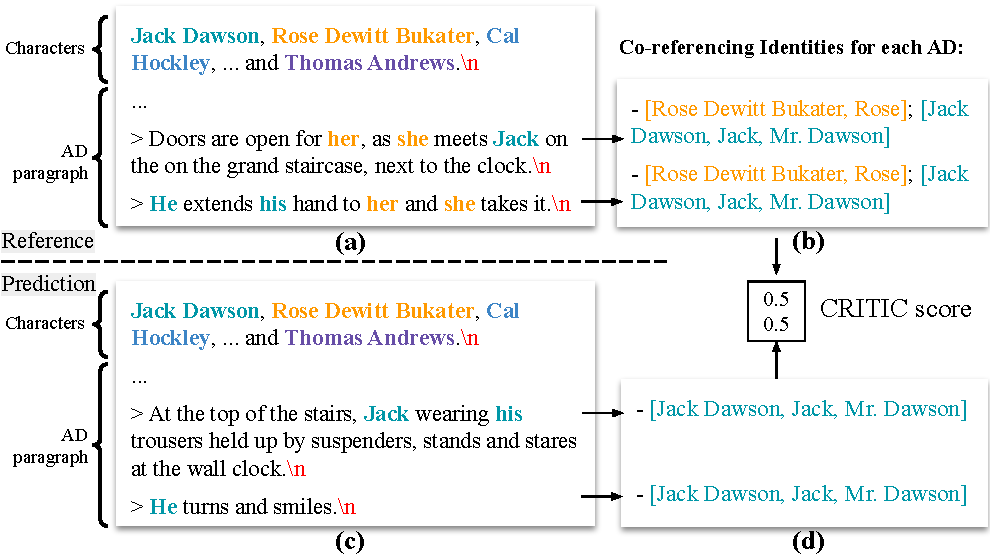
\includegraphics[width=\linewidth]{figs/CRITIC2.pdf}
    \caption{\textbf{CRITIC metric for visual storytelling}. Identities are obtained from character lists and descriptions fed to a co-referencing model. CRITIC \citep{han2024autoadiii} is calculated as the IoU between predicted and reference identities. }
    \label{fig:CRITIC}
\end{figure}

\noindent
\textbf{Dense video captioning}. Dense video captioning approaches generate multiple captions and temporally ground them to corresponding video segments. This is a significantly more challenging task as distinct video segments need to be localized to generate corresponding captions. To localize events in videos, early works \citep{krishna2017dense,li2018jointly,shi2019dense,wang2018bidirectional,zhou2018end} were based on proposal modules from extracted video features. To learn vision-language correspondence explicitly for regions of interest, \citet{zhou2018end} used proposals as masks for visual and language embeddings. Other proposal-based approaches improved proposal generation by using their sequential occurrence as a prior \citep{mun2019streamlined}, feature clipping based on proposals \citep{iashin2020better,iashin2020multi}, or refined general captions for each proposal \citep{deng2021sketch}. Overall, proposal-based methods are optimized on a loss that relates the proposal interval with the ground truth segment, and a captioning loss% that can be formulated similarly to \Cref{eq:captioning}
. As ground truth proposals require exhaustive annotation efforts, more recent efforts have focused on proposal-free approaches. \citet{shen2017weakly} used Multi-Instance Learning (MIL) in which word instances are assigned to bags. They used a binary objective to separate positive bags in which at least one instance corresponds to a target word and negative bags in which no instance contains the target word. MIL has been a building block in subsequent weakly-supervised approaches \citep{chen2021towards}. Further works \citep{yang2023vid2seq,ren2024timechat} have also used sequence-to-sequence modeling with learnable time tokens for visual-language relations. \citet{mavroudi2023learning} combined instruction learning to model the sequentially of video captioning. \citet{islam2024video} used a two-stage autoregressive approach by first generating dense captions for short clips and then cross-attending them to visual features over longer segments to generate longer captions. \citet{zhou2024streaming} aimed at efficiency improvements by compressing frame-instance visual features to clusters.


\noindent
\textbf{Visual storytelling}. A recently introduced challenging task that is gaining interest is the generation of coherent sentences for sequential videos \citep{li2019video}. To bridge cross-modal semantics, \citet{yu2021transitional} used a coherence loss for past, present, and future frames and contrastively pulled visual and language embeddings closer. A similar contrastive objective was used by \citep{xiao2022hierarchical} alongside masking part of the visual input. \citet{han2023autoad} trained a mapping module to project joint CLIP visual features, audio descriptions, and subtitles to an LLM input space to generate captions. Following efforts proposed additional refinements in the pipeline by injecting visual and caption embeddings over multiple LLM layers \citep{han2023autoadii}, using exemplars \citep{han2024autoadiii}, and using character-based prompting \citep{xie2024autoad}. The CRITIC metric, shown in \Cref{fig:CRITIC}, has recently been introduced by \citet{han2024autoadiii} to measure the conceptual alignment of the generated sentences.




\subsubsection{Video Question Answering (VideoQA)}

A widely-used benchmark for VLM models is using visual context to answer textual questions \citep{antol2015vqa,goyal2017making}. In contrast to video captioning, it requires understanding parts of objects and the temporal extent of relevant answers. Depending on the task setting, answers can be obtained from multi-choice QA, or as a global answer in open-end QA. 

%In a multi-choice QA setting, given a video $\mathbf{v}$ and a question $\mathbf{q}$, the goal is to learn a mapping function $\mathcal{F}(\cdot,\theta)$ with $\theta$ parameters to return answer $\mathbf{a}_c \in \mathbf{A}$ from a set of possible answers. In open-end QA settings the answer $\mathbf{a}_c$ is instead generated by model $\mathcal{G}(\cdot,\theta)$ conditioned on the video $\mathbf{v}$ and question $\mathbf{q}$. VQA can take the form:
In a multi-choice QA setting, given a video and a question, the goal is to learn a mapping to return an answer from a set of possible answers. In open-end QA settings, the answer is instead generated from a model conditioned on the video and question. VQA methods can be divided into two broad groups (\Cref{fig:videoqa}).

\begin{figure}[t!]
    \centering
    \begin{subfigure}[t]{0.5\linewidth}
        \centering
        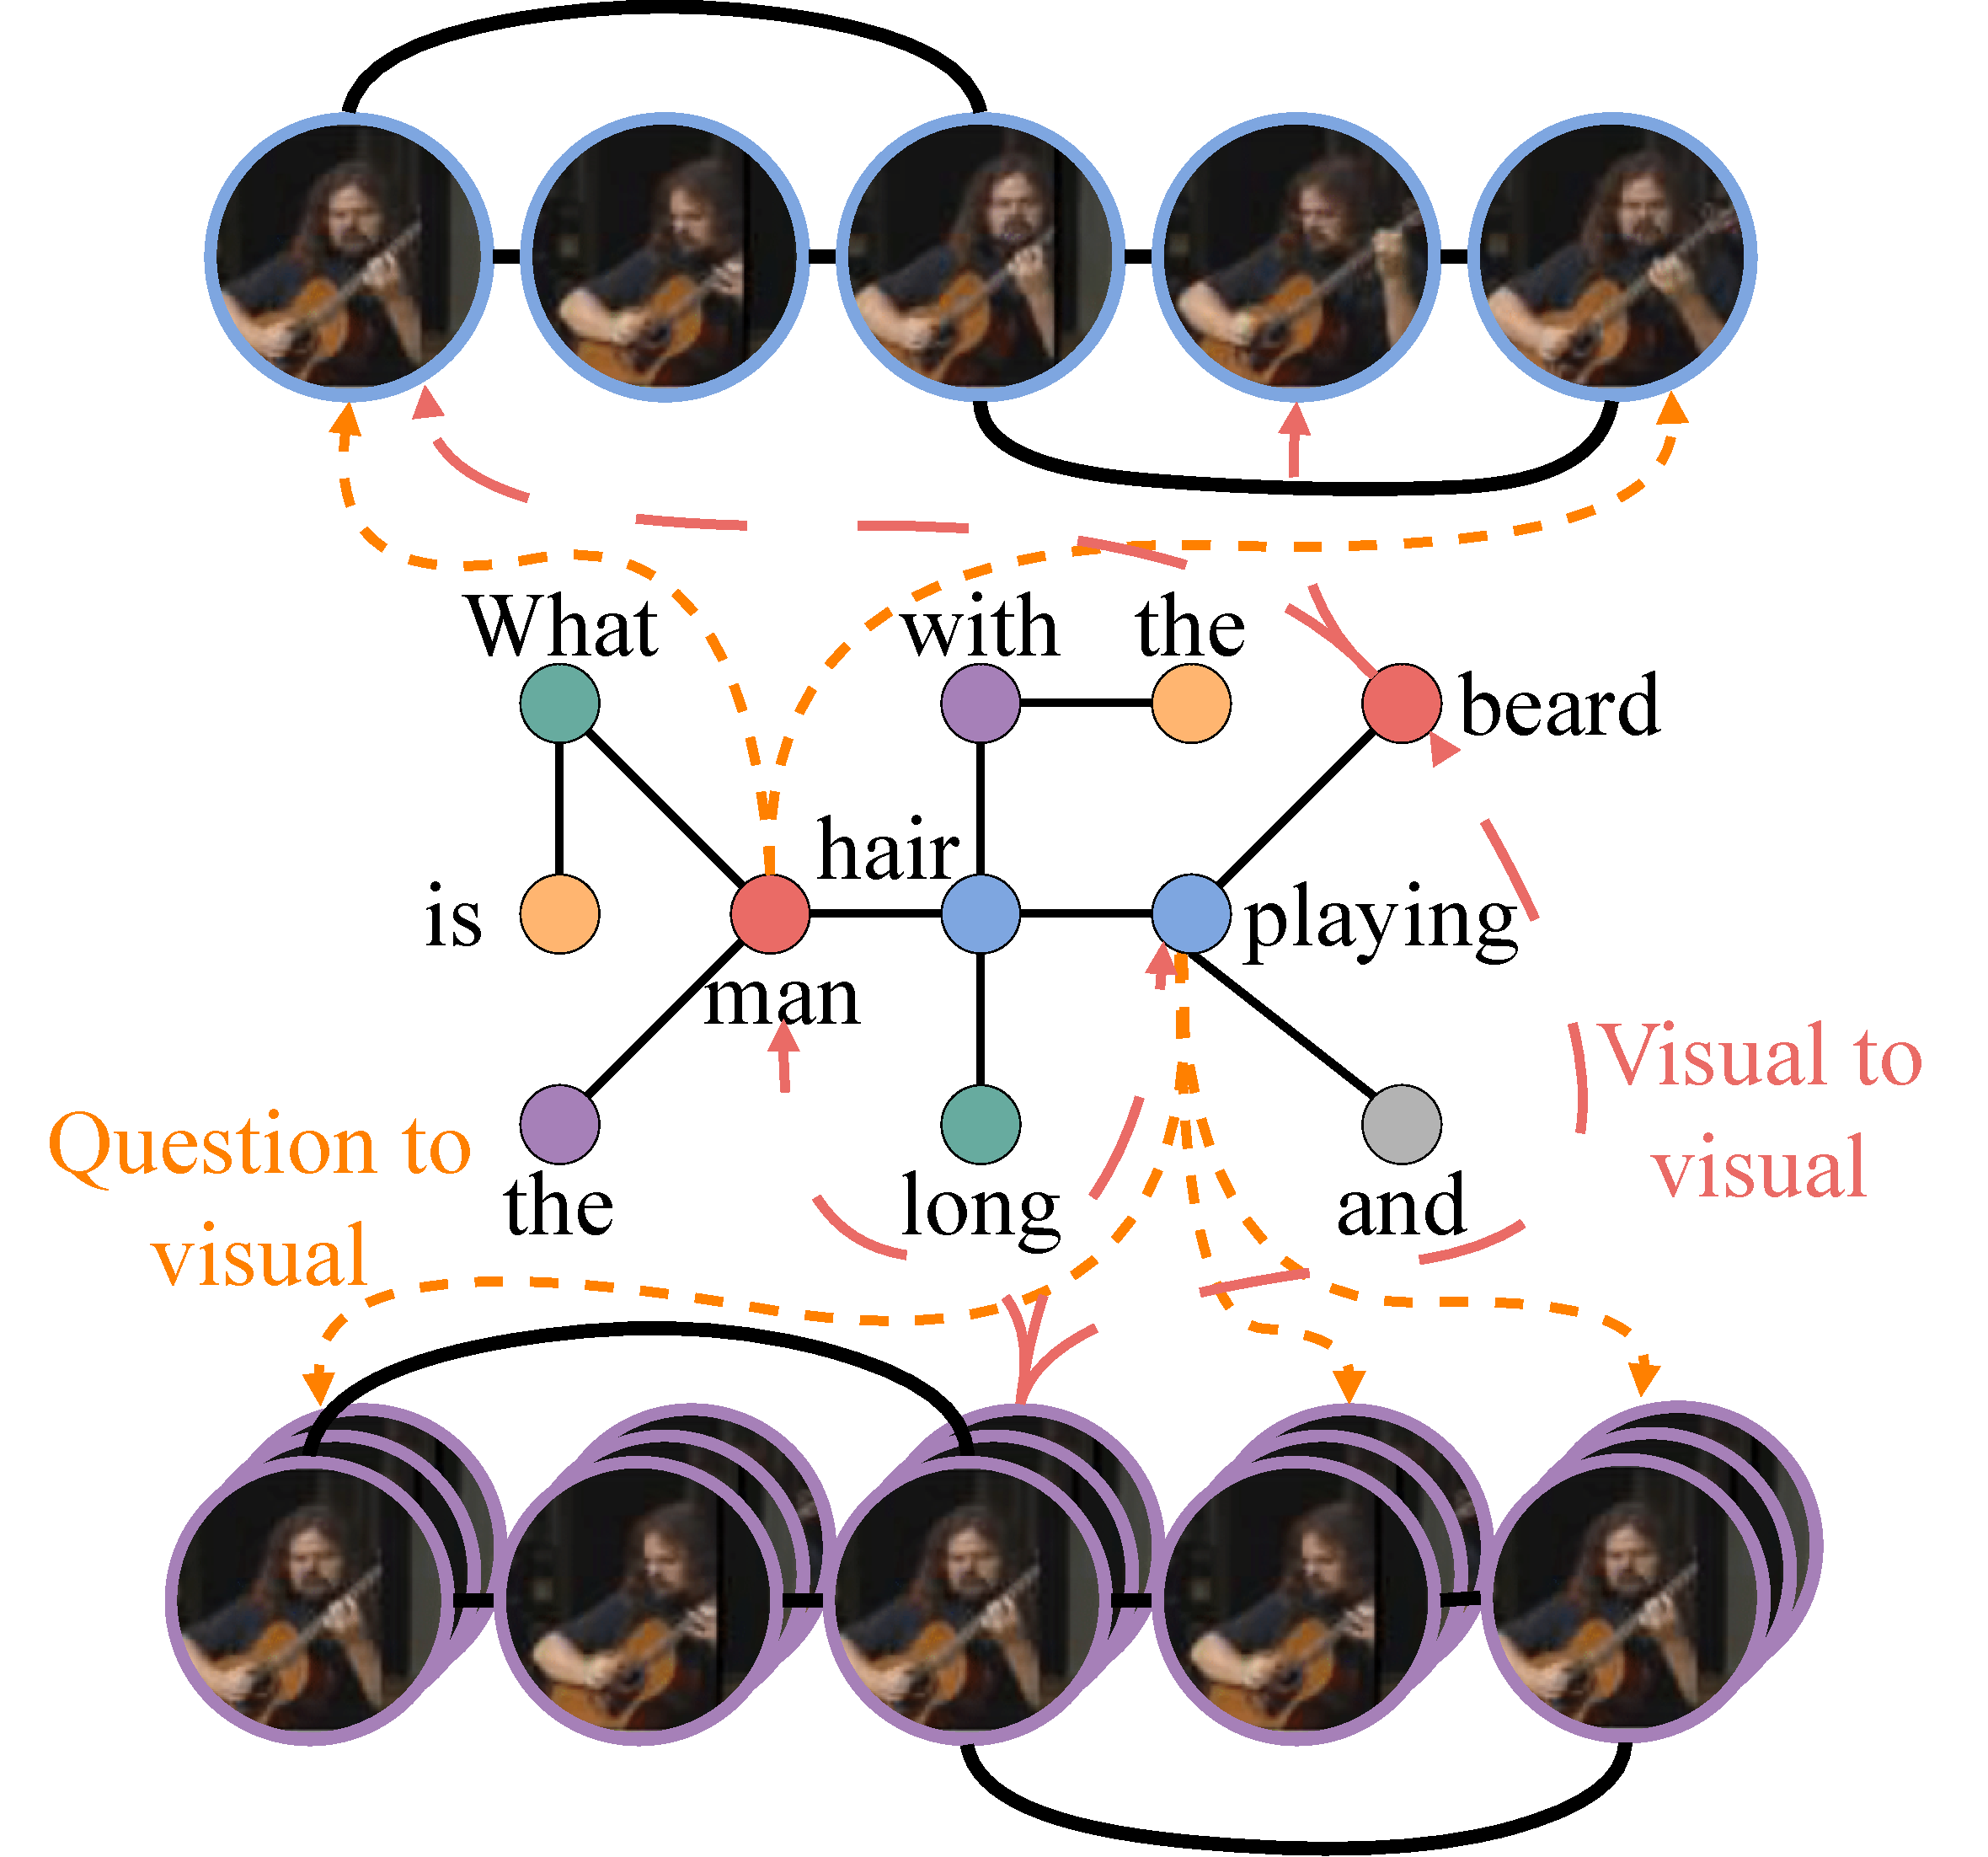
\includegraphics[width=\textwidth]{figs/graph_vqa.pdf}
        \caption{Graph-based}
    \end{subfigure}%
    ~ 
    \begin{subfigure}[t]{0.5\linewidth}
        \centering
        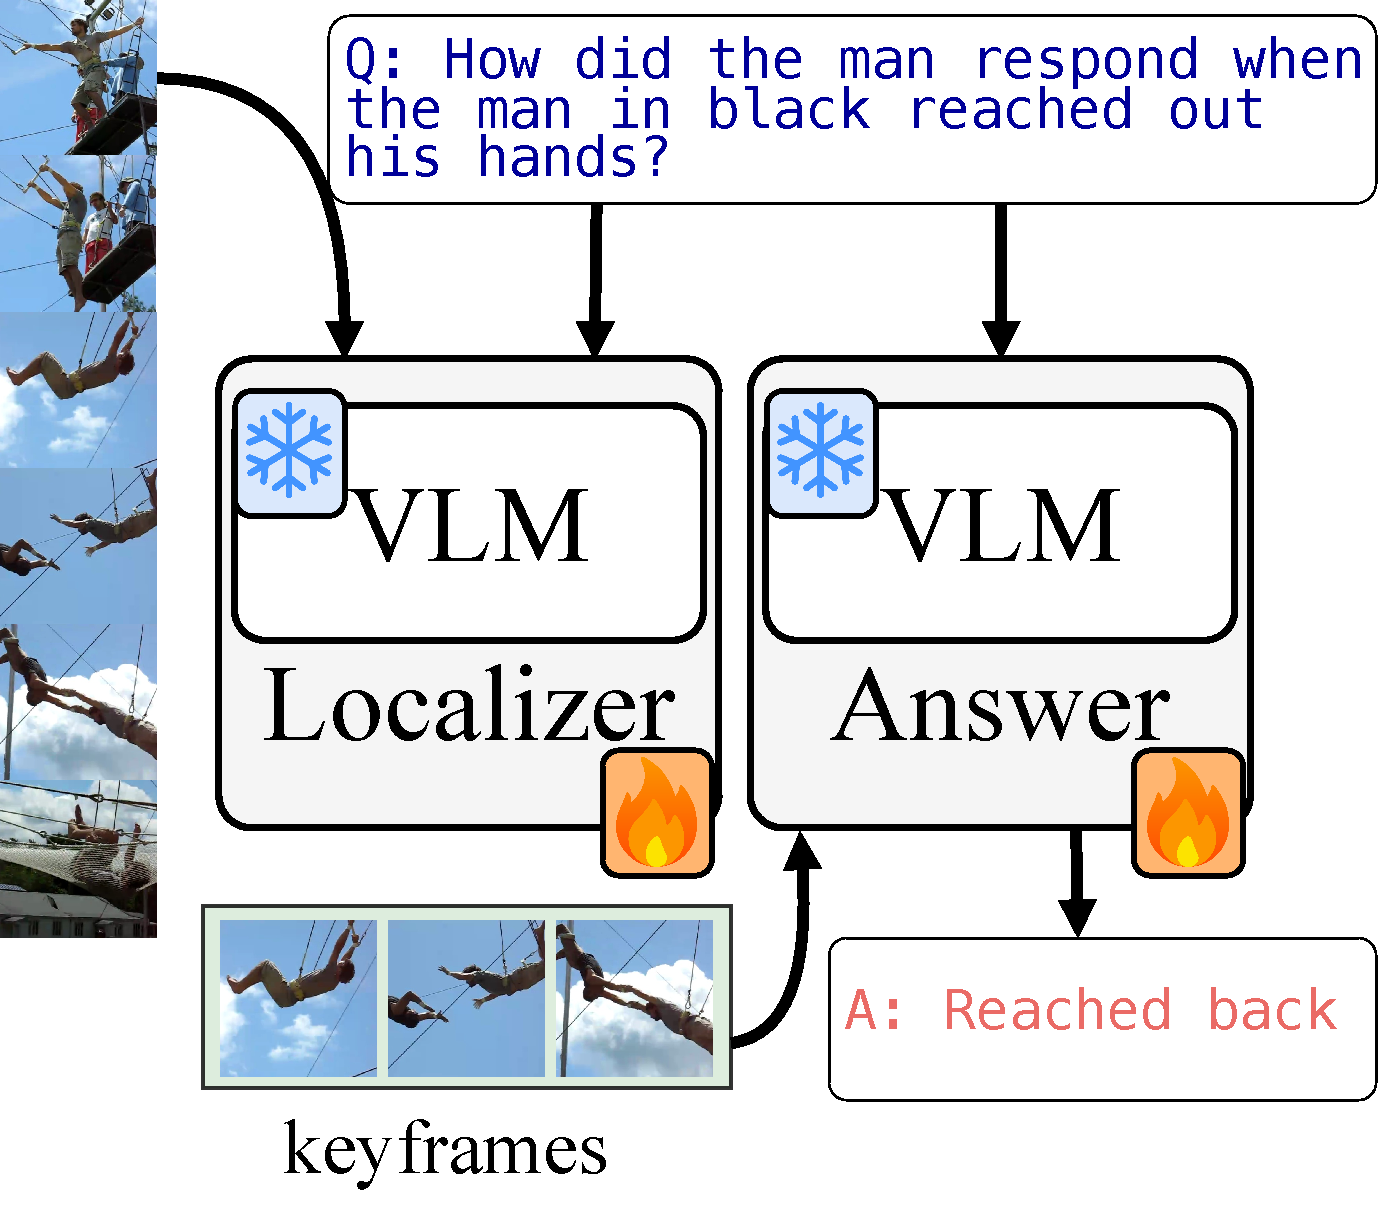
\includegraphics[width=\textwidth]{figs/vlm_vqa.pdf}
        \caption{Memory-based}
    \end{subfigure}
    \caption{\textbf{VideoQA approaches}. The graph-based approach in (a) is based on the method from \citet{park2021bridge}. The memory-based approach with a two-stage VLM in (b) is based on \citet{yu2023self}. Videos sourced from \citet{xiao2021next}.}
    \label{fig:videoqa}
\end{figure}


%\begin{gather}
%    \mathbf{a}_c = 
%    \begin{cases}
%        \underset{\mathbf{a} \in \mathbf{A}}{\text{argmax}} \mathcal{F}(\mathbf{a}|\mathbf{q},\mathbf{V},\theta), \text{if multi-choice QA}\\
%        \mathcal{G}(\mathbf{q},\mathbf{v},\theta), \text{if open-end QA}
%        \end{cases}
%\end{gather}


\noindent
\textbf{Scene-graphs}. Early VideoQA approaches were based on either graph representations \citep{jiang2020reasoning,tu2014joint} or on each modality's heterogeneity. \citet{huang2020location} used object and location-based graph embeddings to relate visual and text features with a cross-modal similarity matrix. Graph representations have also been created from hierarchies of objects and object interactions~\citep{dang2021hierarchical} or over multiple frames~\citep{liu2021hair}. Alternative approaches defined scales from multiple graph convolution resolutions to relate cross-scale interactions \citep{guo2021multi} or from subgraphs to capture static and dynamic scene objects  \citep{cherian20222}. \citet{park2021bridge} created appearance, motion, and question graphs and learned their conditionality by propagating nodes across graphs. Graph representations have also been learned contrastively \citep{xiao2023contrastive} from positive and negative video snippet and answer pairs.


\noindent
\textbf{Multi-modal memory}. Another set of methods aims to memorize relations between visual and text features across time. Initial efforts integrated additional memory modules in LSTMs \citep{jang2017tgif,xu2017video,zeng2017leveraging}. Attention-based approaches \citep{ye2017video} have also been proposed, combining either modality-specific memory modules~\citep{fan2019heterogeneous} or memory-sharing modules cross-attending motion and appearance \citep{gao2018motion,li2019beyond}. Several works \citep{gao2023mist,li2023discovering,yang2022zero,xue2023egocentric} have used a single model with concatenated language and vision tokens to predict answers to queries. Recent approaches have adapted large VLMs for VideoQA. \citet{yu2023self} used a two-stage dual-VLM approach to first localize video segments based on the video and question and then used only the selected frames and question to generate the answer. Similarly, \citet{min2024morevqa} used a list of generated VLM captions describing scenes in videos as input to an LLM. The question was then passed as a prompt to discover the most relevant answer. However, recent works \citep{xiao2024can} reveal that VLM-based approaches may produce answers based on spurious language correlations and not the visual context.


%\citep{yang2022learning}
%\citep{xiao2021next}


\subsubsection{Future outlooks}

Advancements in VLMs have enabled the recognition of actions based on their correspondence to a large lexical corpus. Building upon this correspondence, retrieval, captioning, and question-answering models have moved beyond single instance structural representations and toward the discovery of abstract cross-modal semantics. The increased model capacity provides opportunities for future lines of research.

The majority of VLMs rely strongly on linguistic associations that may not be relevant in vision instances \citep{rahmanzadehgervi2024vision}. A possible alternative is to develop unified multi-modal models in which video frames and images are tokenized in the same manner with positional embeddings also encoding temporal relationships. Initial efforts by \citet{jang2023unifying} and \citet{jin2024integration} have been promising. Another direction includes a better exploration of the objectives used. The majority of works train models on contrastive objectives \citep{chen2020simple,he2020momentum,oord2018representation} which can enforce properties such as feature suppression \citep{chen2021intriguing} and pretext granularity \citep{cole2022does} despite aiming at maximizing correspondence. Crafting better alignment objectives for cross-model representations and semantic relevance can benefit future VLM approaches.  




\subsection{Audio-visual and multimodal recognition} 
\label{sec:recognition::audio}

The recognition of actions or activities has been predominantly studied in the vision domain. In contrast, the auditorily recognition of actions focuses on sounds emitted by objects or actors and their interactions. This task presents distinct challenges as the sounds emitted by different objects or actions can be similar. 

%In developmental psychology, relationships between visual and auditory understanding of the environment are developed at a young age \citep{morrongiello1998developmental}. This has motivated early efforts in active speaker recognition \citep{chen1998audio,matthews2002extraction} and person identification \citep{aleksic2006audio} to study vision and audio cues in tandem.
Time-frequency spectrograms have been a popular format for the representation of audio events in videos. Initial audio-based models have been built following image-based object recognition \citep{gong2021psla} or video classification \citep{kazakos2021slow} CNNs. Attention-based audio methods have used convolutional features \citep{gulati2020conformer,kong2020panns} or image-pre-trained encoders \citep{koutini2021efficient} to attend over spectrogram patches. Approaches have also explored patch masking \citep{baade2022mae,huang2022masked}, focused onsalient sounds \citep{stergiou2023play}, and adapted \citep{liu2022learning_the} or compressed \citep{feng2024coarse} spectrogram resolutions. More recently, the use of audio has gained attention in multi-modal learning settings as it can provide supplementary information to both visual features and language context. 


\subsubsection{Challenges}

The use of multiple modalities introduces several challenges. \textbf{Learning cross-modal dynamics} is a fundamental challenge of multi-modal models as it aims to preserve heterogeneous properties of modalities while maintaining interconnectivity between modalities \citep{liang2022foundations}. Fused embedding spaces \citep{girdhar2023imagebind,girdhar2022omnivore,piergiovanni2023rethinking,zhu2024languagebind} effectively reduce modality-specific information and instead rely on learning a high level of abstraction, with lower heterogeneity and higher interconnectivity. In contrast, modality-specific embedding spaces \citep{gong2022uavm,gong2023contrastive,chen2024soundingactions,recasens2021broaden} are learned through cross-modal associations and rely on effectively transferring distribution across modalities, causing higher heterogeneity and lower interconnectivity. These paradigms are affected by \textbf{domain-specific noise topologies}. Based on a given task or data distribution, the discriminability of each modality differs. Noise naturally occurs based on environment settings, \eg visual features are more relevant in daylight than in night videos. But it can also be observed with instance-based occlusions or sensory imperfections. Such topologies are relevant to developing reasoning structures over modalities \citep{gat2021perceptual}. \textbf{Input representation reasoning} can be defined as combining knowledge from the data and the structure of the objective. Compositional relationships between modalities can be established through concept hierarchies, temporal correspondence, or interactive states. Commonly, such structures are not available beforehand and are instead learned in an unsupervised manner.




\subsubsection{Audio-visual models} 


As video and audio signals differ significantly, works have used two-step models to infer predictions. Two-step approaches extract video and audio embeddings first and then fuse either modality-specific predictions \citep{fayek2020large}, embeddings from multiple modalities \citep{xiao2020audiovisual}, or they jointly attend vision and audio features for the final prediction \citep{gong2022uavm}. More recently, architectures have tokenized and attended audio and vision jointly with multi-modal learnable tokens \citep{nagrani2021attention}, cross-modal attention \citep{jaegle2021perceiver}, and modality gating \citep{xue2023dynamic}. To account for models trained on uni-modal tasks, \citet{lin2023vision} proposed cross-modal adaptors to combine uni-model embeddings in multi-modal tasks. Exploring the relevant audio and visual features with self-supervision has also been a learning paradigm of significant interest. Common embedding spaces can be useful for discovering correspondences in both uni-modal and cross-modal retrieval \citep{arandjelovic2018objects,wu2021exploring}, multi-modal clustering \citep{hu2019deep}, and sound source separation \citep{hu2022mix,mo2023unified,zhao2018sound}. Token reconstruction through masking has also been used as a self-supervised pre-training task with a variety of training schemes including concatenating masked tokens \citep{gong2023contrastive}, multi-view masking per modality \citep{huang2023mavil}, fusing a mixture of per-modality masked tokens \citep{guo2024crossmae}, combining modality-specific masked and unmasked embeddings \citep{georgescu2023audiovisual}, and using multiple masking ratios with siamese networks \citep{lin2024siamese}. 

Variations in the relevance of either visual or auditory signals depend on the instance. A promising direction for integrating this into optimization is gradient blending \citep{wang2020makes} which recalibrates the loss per modality. Other research works have explored multi-audio to single-visual scene correspondence with contrastive learning. This has been done by utilizing joint semantic similarity in both modalities \citep{morgado2021audio}, using active sampling to diversify the pool of negative samples
\citep{ma2021active}, and by counterfactual audio and video pairs to enforce a relationship between multiple audio to single visual scenes \citep{singh2024looking}. Enforcing a similarity constraint between audio and vision steams can also be used to train incremental tasks \citep{pian2023audio}.




\subsubsection{Multi-modal models}

Video is a natural source of multi-modal data. Apart from visual information, audio or textual descriptions can be used in tandem to provide additional signals for actions and events at different granularities. Multi-modal learning has been shown to improve the generalizability of unsupervised models \citep{ngiam2011multimodal} and their generalizability across tasks \citep{paredes2012exploiting}. An initial effort by \citet{kaiser2017one} aimed to create unified multi-modal representations with modality-specific encoders and modality-binding decoders. A similar mixture-of-expects approach was also presented by \citet{munro2020multi} for unsupervised domain adaptation with a dual cross-domain source-target loss over modality pairs. \citet{dai2022one} used sparse activations to train portions of a unified model on specific modalities and tasks. Multi-modal transformers have introduced joint encoder paradigms. \citet{akbari2021vatt} used modality-specific heads to project outputs from a joint audio-text-video encoder trained with a contrastive loss over modality pairs from \citet{miech2020end}. Mixtures of modality-specific encoders and multi-modal head/decoders have also been trained with masking tokens \citep{zellers2022merlot}, adding cross-modal attention blocks in the encoder \citep{recasens2023zorro}, using an ensemble of uni-modal teachers \citep{radevski2023multimodal}, and adding vision and audio projectors for LLM heads \citep{zhang2023video}. \citet{zhang2024multimodal} introduced features from different modalities to the multi-modal head at different training steps capturing cross-modal associations iteratively during training. \citet{srivastava2024omnivec} included meta tokens to represent modality dimensions and channels to embed modality-specific features in a common space. This was further adjusted \citep{srivastava2024omnivec2} to also cross-attend joint-embedded features and uni-modal features.





\subsubsection{Future outlooks}

Most current multi-modal models rely on the availability of all modalities at the start. New models are re-trained when additional modalities are added. A promising direction would be to design adaptive models that integrate unseen modalities more efficiently \citep{ma2022multimodal}. This has been explored by recent methods by transferring seen to unseen modality distributions \citep{wang2023distribution}, cross-attending over unseen modalities \citep{recasens2023zorro}, aligning uni-modal and multi-modal features in training \citep{zhang2023learning}, using modality-specific adapters \citep{lin2023vision}, and predicting missing modality features with learnable tokens \citep{kim2024missing}. Learning adaptable models that can process inputs in new modalities at inference time not only benefits performance for specific tasks but also enables advancement in more general tasks such as online learning \citep{bottou1998online}, incremental learning \citep{schlimmer1986case,utgoff1989incremental}, and federated learning \citep{konevcny2016federated}.




%\subsection{Interaction recognition}
%\label{sec:recognition::interaction}

%\noindent
%\textbf{Dyadic human-human interactions}

%\citep{nguyen2024hig}
%\citep{ong2023chaotic}

%\noindent
%\textbf{Group interactions}

%\noindent
%\textbf{Human-object interactions}